\documentclass[12pt,a4paper,twoside,openright]{book}

%--- imported packages in alphabetical order ---%
\usepackage{acro} % acronyms (acsetup, list of abbreviations)
\usepackage[toc,page]{appendix}
\usepackage[hyphenbreaks]{breakurl}
\usepackage[english]{babel}
\usepackage[numbered]{bookmark}
\usepackage{caption}
\usepackage{color}
\usepackage{dirtree} % directory structure
\usepackage{fancyhdr}
\usepackage{geometry}
\usepackage{graphicx}
\usepackage{hyperref}
\usepackage[utf8]{inputenc}
\usepackage{listings}
\usepackage{mdwlist} % itemize with reduced spacing
\usepackage{pdfpages}
\usepackage{scalerel} % inline text image
\usepackage{subcaption}
\usepackage{url}
\usepackage{xcolor}

%--- unused packages ---%
% \usepackage[T1]{fontenc}
%\usepackage{times}
% \usepackage{forest}
% \usepackage[nottoc]{tocbibind}
% \usepackage{syntonly}

% makes latex quickly check the document, runs faster and saves time
%\syntaxonly


\geometry{
	portrait,
	bindingoffset=1.5cm,
	inner = 2.5cm,
	outer = 2.5cm,
	top = 3cm,
	bottom = 2cm,
}


\pagestyle{fancy}
\fancypagestyle{myStyle}{
    \fancyhf{} % clear all header and footer fields
    \fancyhead[LE,RO]{\leftmark}
    \fancyhead[RE,LO]{\thepage}
    \renewcommand{\chaptermark}[1]{\markboth{\thechapter. {\slshape{##1}}}{}}
}


\linespread{1.5}


\graphicspath{ {img/} }


\hypersetup{%
	bookmarks = true, % show bookmarks
	unicode = true, % non-Latin characters
	pdftitle = {Master Thesis}, % pdf title
	pdfsubject = {Creating a website with Info-Terminal and Live CCTV Stream for the Smart Home%
		Laboratory at Hochschule Furtwangen University},%
	pdfauthor = {Ashiq Mohamed Akbar Ali},%
	pdfkeywords = {master}{thesis}{website}{info}{terminal}{live}{cctv}{stream}{smart}{home}%
		{laboratory}{ashiq}{mohamed}{akbar}{ali}{hochschule}{furtwangen}{university}{hfu}{ss}%
		{2017},%
	pdfcreator = {pdflatex},%
	pdfproducer = {LaTeX},%
	colorlinks = true, % true:colored links; false:boxed links
	linkcolor = black, % links font-color
	urlcolor = black, % url font-color
	linkbordercolor = white, %links border-color
	urlbordercolor = white, % url border-color
	citecolor = black,
	citebordercolor = white
}


%--- lst listing / enviroments for code setup ---%
\lstset{
	aboveskip=3mm,
	belowskip=3mm,
	basicstyle=\footnotesize,
	breaklines=true,
	tabsize=3,
	breakatwhitespace=true,
	frame=l
}


%--- acronyms / list of abbreviations setup ---%
\acsetup{first-style=short}


%--- document information ---%
\title{Master Thesis}
\author{Ashiq Mohamed Akbar Ali\\Mobile Systeme\\252641}
\date{SS 2017}



\DeclareAcronym{html}{
	short = HTML,
	long = HyperText Markup Language,
	class = abbrev
}
\DeclareAcronym{css}{
	short = CSS,
	long=  Cascading StyleSheet,
	class = abbrev
}
\DeclareAcronym{js}{
	short=JS,
	long=JavaScript,
	class=abbrev
}
\DeclareAcronym{php}{
	short = PHP,
	long = Hypertext Preprocessor,
	class = abbrev
}
\DeclareAcronym{iot}{
	short=IoT,
	long=Internet of Things,
	class=abbrev
}
\DeclareAcronym{ip}{
	short=IP,
	long=Internet Protocol,
	class=abbrev
}
\DeclareAcronym{lan}{
	short=LAN,
	long=Local Area Network,
	class=abbrev
}
\DeclareAcronym{wlan}{
	short=WLAN,
	long=Wireless Local Area Network,
	class=abbrev
}
\DeclareAcronym{cctv}{
	short=CCTV,
	long=Closed Circuit Television,
	class=abbrev
}
\DeclareAcronym{cms}{
	short=CMS,
	long=Content Management System,
	class=abbrev
}
\DeclareAcronym{http}{
	short=HTTP,
	long=HyperText Transfer Protocol,
	class=abbrev
}
\DeclareAcronym{cgi}{
	short=CGI,
	long=Common Gateway Interface,
	class=abbrev
}
\DeclareAcronym{ssid}{
	short=SSID,
	long=Service Set Identifier,
	class=abbrev
}
\DeclareAcronym{uri}{
	short=URI,
	long=Uniform Resource Identifier,
	class=abbrev
}
\DeclareAcronym{ajax}{
	short=AJAX,
	long=Asynchronous JavaScript,
	class=abbrev
}
\DeclareAcronym{api}{
	short=API,
	long=Application Programming Interface,
	class=abbrev
}
\DeclareAcronym{2d}{
	short=2D,
	long=2 Dimensional,
	class=abbrev
}
\DeclareAcronym{3d}{
	short=3D,
	long=3 Dimensional,
	class=abbrev
}
\DeclareAcronym{sftp}{
	short=SFTP,
	long=Secure File Transfer Protocol,
	class=abbrev
}
\DeclareAcronym{nginx}{
	short=Nginx,
	long=Engine X,
	class=abbrev
}
\DeclareAcronym{wp}{
	short=WP,
	long=WordPress,
	class=abbrev
}
\DeclareAcronym{url}{
	short=URL,
	long=Uniform Resource Locator,
	class=abbrev
}
\DeclareAcronym{cdn}{
	short=CDN,
	long=Content Delivery Network,
	class=abbrev
}
\DeclareAcronym{vm}{
	short=VM,
	long=Virtual Machine,
	class=abbrev
}
\DeclareAcronym{ssh}{
	short=SSH,
	long=Secure Shell,
	class=abbrev
}
\DeclareAcronym{rdbms}{
	short=RDBMS,
	long=Relational Database Management System,
	class=abbrev
}
\DeclareAcronym{sql}{
	short=SQL,
	long=Structured Query Language,
	class=abbrev
}
\DeclareAcronym{tcp}{
	short=TCP,
	long=Transmission Control Protocol,
	class=abbrev
}
\DeclareAcronym{udp}{
	short=UDP,
	long=User Datagram Protocol,
	class=abbrev
}
\DeclareAcronym{xss}{
	short=XSS,
	long=Cross Site Scripting,
	class=abbrev
}
\DeclareAcronym{seo}{
	short=SEO,
	long=Search Engine Optimization,
	class=abbrev
}
\DeclareAcronym{rss}{
	short=RSS,
	long=Rich Site Summary,
	class=abbrev
}


\begin{document}
\frontmatter

\pagestyle{empty}
\bookmark[page=1,level=1]{Title Page}
\begin{titlepage}

\begin{flushright}
	
\includegraphics[width=4.5cm,height=1.5cm]{titlepage/hfu.png}
\end{flushright}
	
\begin{center}

	%--- Bachelor or Master Thesis ---%
	\vspace{1cm}
%	\rule{\linewidth}{0.2mm}\\[0.4cm]
	\huge
	\textbf{Master Thesis}\\
%	\rule{\linewidth}{0.2mm}\\[0.4cm]

	\vspace{1.25cm}
	\Large

	%--- thesis title ---%
	Creating a website with Info-Terminal and Live CCTV Stream for the Smart Home Laboratory at
	Hochschule Furtwangen University

	\vspace{0.75cm}
	by
	
	%--- author name ---%
	\vspace{0.75cm}
	Ashiq Mohamed Akbar Ali\\
	252641

	\vfill

	%--- information ---%
	\large
	A thesis submitted for the degree of\\
	Master of Science

	\vspace{0.1cm}
	in

	\vspace{0.1cm}
	Mobile Systeme

	\vspace{0.5cm}
	%--- faculty name ---%
	Faculty of Computer Science\\
	%--- university name ---%
	Hochschule Furtwangen University

	\vspace{0.5cm}
	Supervisor: Prof. Dr. Elmar Cochlovius\\
	Co-Supervisor: Judith Jakob, M.Sc.

	\vspace{0.5cm}
	Summer 2017

	\end{center}
\end{titlepage}

%\pagenumbering{Roman}

\pagestyle{plain}

\chapter{Abstract}
In the era of the Internet, it has became a norm or to an extend very much required for every institution to make its presence through a website. The Smart Home Laboratory at Hochschule Furtwangen University is not an exception. The laboratory, which is under renovation, is nearing its completion and is expected to be fully functional soon. Hence, this laboratory requires a website that will let the public to learn more about the laboratory through the information provided on this website. This website is built by using WordPress content management system. On top of that, it has been developed with an Info-Terminal --- an automated slide show --- that will give an insight about the laboratory interactively to the visitors. This website also has been programmed to stream live footage of an IP Camera, that is mounted in the laboratory. Through this thesis, a few websites of smart home labs of other institutions have been researched and available plugins in the WordPress marketplace has been analyzed, in order to create and design the Info-Terminal. This thesis also outlines the implementation steps for the tasks involved in the development process right from the beginning till the end.

\vspace{12pt}
\noindent
Keywords: Smart Home Lab, Website, WordPress, Info-Terminal, Live CCTV Stream
\chapter{Acknowledgement}

All praise to God --- the Creator, the Nourisher, the Cherisher, the Sustainer and the Provider.

Before I could even started with my thesis work itself, I required helps and supports of others. As no one one can stand alone on his own, as he continually requires the help and support of others, it is important to thank them and appreciate their gratefulness. In my opinion, the thanks we give to others don't equates to the help, support and encouragement they have given. But what I do believe is our thanks will encourage them to continue their help to others without a period.

By saying that, I would like to thank foremost my professor as well as my supervisor, Prof. Dr. Elmar Cochlovius for an interesting thesis topic. Without his help and supervising, this thesis wouldn't have been possible. His continual support and feedback have helped this work to take its course and shape in the last six months. And my second supervisor, Miss Judith Jakob, for her support and encouragement through out this thesis work.

Next, I would like to thank my friends and acquaintances and housemates - Suprita, Bhargav, Preethi, Noor, Darshan, Siva, Subbu, Sachin, Mati, Alex, Deshi, Max, Mothanna, Omar, and Muhammad. They have helped and encouraged me in so many ways and for so many days. I owe them all a lot which I cannot repay. 

Lastly, I want to thank my parents and siblings. For their patience and understanding in letting me pursue my dream.

\tableofcontents

\cleardoublepage % so that page number reference is correct
\addcontentsline{toc}{chapter}{\listfigurename}
\listoffigures


\cleardoublepage
\addcontentsline{toc}{chapter}{\listtablename}
\listoftables


\chapter{List of Abbreviations}
\printacronyms[include-classes=abbrev,name=]


\mainmatter
\pagestyle{myStyle}
%\pagenumbering{arabic}
\chapter{Introduction}

The Smart Home Laboratory has been established at Hochschule Furtwangen University, Campus Furtwangen a few years ago. This laboratory can be found at B2.01. Currently, this laboratory does not have an official website yet. Hence, through this master thesis, a website has to be created by using the \ac{cms}, called WordPress.

This website allows the university's professors and students, as well as public to access and learn about the smart home lab interactively through any web browsers. In order to achieve that, the website will be equipped with an Info-Terminal, which will display all the available systems, devices, as well as sensors and actors in the lab.

Here is a description of Info-Terminal. The Info-Terminal is an automated tour i.e. endless presentation. It will provide information regarding the components, panels and use cases in the Smart Home Laboratory. Additionally, it has controllers such as play, pause, next, previous and home buttons. Other than than, there are thumbnails at the bottom to navigate and view all the slides available in the info terminal. This will allow the users to have an overview of the smart home laboratory and navigate it interactively.

Other than that, a live stream of CCTV recording has been programmed and added to the website. This CCTV can be found in the lab. The website enables the privileged users to view live recording through the website. In addition to that, a 3D-Model made through the Unity technology has been integrated into the WordPress.

The Info-Terminal has to be programmed as such that it can be viewed through a touch display called Microsoft Surface Hub, which can be found in the lab. Though the website as well as the Info-Terminal has been programmed and designed to be viewable across all devices, it has been a little more consideration to be best suited on the Microsoft Surface Hub.

\section{Aim and Objectives}
The main aim of this master thesis is to create a website using WordPress, which contains Info-Terminal and displays live CCTV recordings.

Here is an overview of objectives that has been achieved in this thesis work:
\begin{itemize*}
\item Preparation of expose, documentation structure, literature sources, time-planning and calendar-planning
\item Research on smart home lab websites and contents of other universities
\item Server setup and installation of WordPress
\item Tutorials on WordPress, its theme and plugins
\item Structuring, designing and adding the contents to the website
\item Building the Info-Terminal based on the systems and devices available in the lab.
\item Connecting CCTV recording to the website
\item Integrating 3D Unity model
\item Setting up email server
\item Ensuring security and safety of the server and the website
\end{itemize*}

\section{Project Management}
The thesis has to be done in six months period. It has been started on the first of March and has to completed and submitted by the end of August 2017. This includes finishing up the practical part and the documentation on it.

The thesis is started officially with creating expose and defining aims as well as constructive objectives. At the beginning stage, the project management part for this thesis has been planned. As planned, status reports and thesis planning has to be submitted every two weeks on the odd calendar week. Other than that, meeting and discussions have been held every four weeks to discuss on the outcome and further works that has to be carried out.

In the project management phase, the time planning and calendar planning has been organized accordingly with the tasks that has to be carried out through out six months time period. Before the implementation of website has been started, context diagrams has been created as a summarization of the practical tasks that were to be done. Apart from that, the contents for the documentation has been structured to mediate the report writing at the later stage.

\section{Documentation}
This documentation consist of following chapters:
\begin{description}
\item[Chapter 2] discusses the related background works and researches
\item[Chapter 3] outlines the ideas and approaches involved in solving the problem
\item[Chapter 4] discusses the technologies used in order to create the website
\item[Chapter 5] explains the server setup and installation of required software
\item[Chapter 6] shows the important steps involved in designing the website
\item[Chapter 7] shows steps involved in creating Info-Terminal
\item[Chapter 8] outlines on work involved in streaming CCTV live recording
\item[Chapter 9] shows how to integrate 3D unity model into a WordPress powered website
\item[Chapter 10] explains step-by-step on how to enable blogging on the website
\item[Chapter 11] summarizes this thesis work with future outlook
\end{description}
\chapter{Background Works}
The background works involved in this thesis in order to create the Smart Home Lab website divided into two parts. The first part is the analysis of selected Smart Home Lab websites of other institutions. The second part is the analysis of the WordPress plugin in order to create the Info-Terminal.

\section{Website Analysis}
In this work, altogether six websites have been analyzed. These include FZI Forschungszentrum, KIT iZEUS, IoTLab Reutlingen, Duke Smart Home Program, MIT Mobile, and MIT Smart Living. In general, criteria such as the layout, contents, main navigation menu, media supported, responsiveness and languages supported have been analyzed.

\subsection{FZI Forschungszentrum}

\subsubsection*{Website Information}
\begin{itemize*}
\item URL: https://www.fzi.de/en/home/
\item Web server: Apache
\item Application server: PHP 5.4.45
\item CMS: Typo3
\end{itemize*}

\subsubsection*{Web Layout}
The website uses normal layout, not screen-wide. The theme look modern, but the normally used one. The Header contains institution logo on the right, and the top part has option to change language, link to contact page and search bar. Lower part of the header has main navigation menu (Home, News, Research, Our Offer, Work For Us, and About Us). The header is fixed, but collapse when user scroll down.

Body is two column sized. In all pages except home page, the small left column has sub menu respective to that individual page and large right column has the content. On the main page, the the left column is relatively bigger which has slideshow and latest news feed. Right column is relatively small and has list of upcoming events and quicklinks.

Footer is small sized. It has sub menu on the left (Home, Privacy, Legal Notice, Sitemap, Search) It also has social media plugins on the (Xing), \ac{rss} feeds and contact links.

\subsubsection*{Contents}
Contents presented on the website are the home page (featured article/news, upcoming events, latest news, quicklinks), newsfeed, research (research sector, research focuses, projects etc), offers, work for us (carrier page), about us, privacy, legal notice, and sitemap. As analyzed, the website has a lot of contents, perhaps it could have been organized in a better way.

\subsubsection*{Menu}
There are 3 types of menu:
\begin{itemize*}
\item Main navigation menu situated at the header (Home, News, Research, Our Offer, Work For Us, and About Us)
\item Sub menu respective to individual pages which is different from one another located at right column of the body part
\item Footer menu located the footer (Home, Privacy, Legal Notice, Sitemap, Search).
\end{itemize*}

\subsubsection*{Media}
The website supports the following medias, such as images, slide show, videos, contact form, search bar, social media button.

\subsubsection*{Responsiveness}
The web page is responsive. The header is compressed. The main navigation menu is shifted to the bottom of the page with a link to the menu located at the header. The two column body part is changed to single column on window resize. The sub menu on the individual pages are merged with main navigation menu in hierarchical order, which is situated at the bottom of the page.

\subsubsection*{Languages}
The website supports German and English languages.

\subsection{KIT iZEUS}
\subsubsection*{Website Information}
\begin{itemize*}
\item Url: http://www.izeus.kit.edu/62.php
\item Web server: Apache 2.4.10
\item Application server: PHP
\item Server: Debian
\end{itemize*}

\subsubsection*{Web Layout}
The web layout is classic normal one. It is not wide and not stretched. The institution logo is located in the header at the top. The sub-menu can be spotted small in the upper right part of the header. The main frame is divided into three columns. The left column contain the main navigation menu. The center column serves as the main content. Lastly, the right column fixed banner. The footer is small and has copyright statement.

The web layout is classic without fancy popup animations, graphics, slider etc. It has to also noted that it is most common and user friendly where most users know how to navigate.

\subsubsection*{Contents}
Contents presented on the website are the home page, energy smart home lab, information materials, project consortium (partners and KIT chairs), publications, press review, links, contact, legals and sitemap. The content look organized, clear to be viewed and read. Navigating through the contents is also easy, but it appears not to be updated anymore.

\subsubsection*{Menu}
The website contains two menus:
\begin{itemize*}
\item Small top right menu (Home, Lang Pref, Legals, Sitemap, Link to KIT)
\item Main Menu on Left Column (Home, Energy Smart Home Lab, Information Material, Project Consortium, Publications, Press Review, Links, Contact)
\end{itemize*}

Analysis: Both navigation are visible on all pages, static, easy to use, simple hovering effect, highlight on active link.

\subsubsection*{Media}
The website supports the following media, video, images, banners, PDFs, and external links. However, no animation, picture gallery and image slider can be spotted.

\subsubsection*{Responsiveness}
The website is not responsive. It is best viewed with desktop and laptop. Having said that, it is not mobile- or tablet-friendly and not recommended for Microsoft Surface Hub.

\subsubsection*{Languages}
The website has German as the primary language and supports English as an alternative language. The website is designed will on both the languages.

\subsection{IoTLab Reutlingen}
\subsubsection*{Website Information}
\begin{itemize*}
\item URL: http://iotlab.reutlingen-university.de
\item Web server: Apache
\item Application server: PHP 5.5.36
\item CMS: Joomla!
\end{itemize*}

\subsubsection*{Web Layout}
The website uses a modern web layout and the web page is full-width stretched. The header contains brand logo and horizontal main navigation menu. The header also contains toggle button to open / close main navigation menu. It is fixed and the both menus are duplicated.

The website is created using Joomla! content management system. The home page is single columned with newsfeed. Whereby, the other pages are double column, with right column containing sub-menu and left column showing the main content. Other that that, fixed social media icons (e.g. facebook and twitter) can be found on right edge of the website.

The footer contains copyright statement, impressum link, link to university homepage, link and info about CMS, and link / info about CMS theme. The web layout doesn't look systematic and well organized even though 
it uses modern web templating. The users might face difficulty to get  information or contents they are looking for.

\subsubsection*{Contents}
The website contains the contents such as new feeds on home page, master projects listing (current and finished master projects, team , introduction), publications, thesis, blogs (containing 3 categories: IoTLab-Blog, Mobile Computing and Distributed), systems, contact form, and commenting for blog article.

\subsubsection*{Menu}
The website has three menus:
\begin{itemize*}
\item One menu located on the web page header (Home, Master Project, Publications,  Thesis, Blog), but Hidden on mobile / tablet mode.
\item Sidebar Menu which has to be toggle opened/closed using button (Duplicate of  the main menu located on the header with additional menu "Intern")
\item Menu located at left column of pages (Duplicate of the menu with some  additional menus such as Cooperation, News, Events etc.)
\end{itemize*}

The menus are duplicated which is inconvenient and confusing for the user to navigate around.

\subsubsection*{Media}
The website contains images, slide shows, and video. It also supports PDFs, banner and animation.

\subsubsection*{Responsiveness}
The website is responsive and adapts to various screen sizes. The contents are readable and viewable using different devices. It is mobile- and tablet-friendly.

\subsubsection*{Languages}
The website supports only English language.

\subsection{Duke Smart Home Program}
\subsubsection*{Website Information}
\begin{itemize*}
\item URL: https://smarthome.duke.edu/
\item Web server: Apache 2.4.7
\item Application server: PHP 5.5.9-1
\item CMS: Drupal 4.7
\item Server: Ubuntu 4.20
\end{itemize*}

\subsubsection*{Web Layout}
The website uses modern yet simple web layout. The web page is fill-width stretched. The header is divided into three layers. The first layer is smallest and contains two external links. The second layer big and has brand logo and search bar. And the third layer is smaller and has main navigation menu.

The main view of website is divided into two columns. The left column is the main column containing contents. The right column is small and has sub-menu respective to each pages. The footer part is medium sized contains copyright statement, institution logo and a link to contact us.

For analysis, in overall web design looks fine, but unable to scroll through the page using scroll wheel.

\subsubsection*{Contents}
The website consists of following pages. The home page contains picture, about the program, links targeted to different audience, 3 recent research projects. Other that that, there are about, research, out smart dorm, industry, students and contact us pages. The contents are well presented and organized.

\subsubsection*{Menu}
Two types of menu:
\begin{itemize*}
\item Main navigation menu located at the header of the website (About, research, our smart dorm, industry, students, contact us)
\item Sub-menu different for individual pages located at right column next to the main layout.
\end{itemize*}

The menu are well located and easy for the user to navigate.

\subsubsection*{Media}
The website has images, video, map and banner. However, no gallery, slider and contact form can be spotted.

\subsubsection*{Responsiveness}
The website is fully responsiveness and mobile-friendly. The main navigation menu appears as a left drawer which can be toggled opened and closed.

\subsubsection*{Language}
English is the primary and the only language offered by this website.

\subsection{MIT Mobile Experience Laboratory}
\subsubsection*{Website Information}
\begin{itemize*}
\item URL: http://mobile.mit.edu
\item Web server: Apache 2.2.22
\item Application server: PHP 5.4.45
\item CMS: WordPress 4.3.1
\item Theme: WordPress Construct (MEL Edition)
\item Server: Debian 7u8
\end{itemize*}

\subsubsection*{Web Layout}
The website use a modern web layout. It is wide screen but not stretched. The contents are arranged in tile-based design. The header contain the institution logo with home page link. The main navigation menu can be found on the header as well.

The main layout is single columned. It has breadcrumb at the top part of the main layout. The projects and event+classes pages have filtering option on the left side. The main navigation menu in the footer is a duplicate from the header' menu. The footer also contains copyright statement, institution and department logo containing external links to their website respectively.

The look of the website is different than normal website as all the contents are arranged in the tiled format.

\subsubsection*{Contents}
The main page contains featured news, upcoming recents+classes, short introduction and contact us section. Other than that, the pages as such, about us, projects that can be filtered according to topic, events+classes that can be filtered according to month/year, team members and sponsors can be found on this website.

\subsubsection*{Menu}
The are two menus on this website:
\begin{itemize*}
\item Main navigation menu located at the header (Home, about, projects, events+classes, team, sponsor)
\item Footer menu, same as the main navigation menu
\end{itemize*}

The menu looks simple, decent, easy to navigate and direct forward.

\subsubsection*{Media}
The website supports all normal media files. Additionally, slide show, images that can be zoomed-in, breadcrumb, and project has 'related projects' link.

\subsubsection*{Responsiveness}
The website is not responsive as tested. It is not scaling to fit the size of mobile and tablet screens. The user as to browse the website in desktop mode in the mobile devices.

\subsubsection*{Languages}
The website supports only English as primary and the only language.

\subsection{Avea Smarthomes Re:Thinking}
\subsubsection*{Website Information}
\begin{itemize*}
\item URL: http://mobile.mit.edu/smartliving/
\item Web server: Apache 2.2.22
\item Application server: PHP 5.4.45
\item CMS: WordPress 4.3.1
\item Theme: WordPress Time (Smart living edit)
\item Server: debian 7u8
\end{itemize*}

\subsubsection*{Web Layout}
The web layout of this website looks modern. It is wide but not stretched. The header has two section. First, a broad section for brand logo centralized. Second part has the main navigation menu. The main layout of website is single columned with simple layout. The footer contains copyright statement centralized.

The website has a simple web interface without much fancy items.

\subsubsection*{Contents}
The website has the following pages, home page with slide show, project brief containing project introduction, methodology and projects listing (FLOC, SOL-CHARGE, BOX OF HOLDINGS, COOKBOX.NET) and team.

\subsubsection*{Menu}
There is only one main navigation menu at the header:

\subsubsection*{Media}
The website contains media such as images, slide show and video.

\subsubsection*{Responsiveness}
The website is responsive, but some of the elements could be positioned well (e.g. header). The main navigation menu becomes as a drop down list in the tablet and mobile mode. Since the web page is single column, there is not much change in the body part.

\subsubsection*{Languages}
The website supports only English language.


\section{WordPress Plugins Analysis}
The Info-Terminal has been created with a WordPress plugin. Among many available plugins, slider is a great option to create a stunning gallery of slides containing images, texts, buttons, video etc. There are plenty slider plugins available in the WordPress plugin marketplace. This section will summarize the analysis of the slider plugins that have been tested.

Even though more than 10 plugins have been installed and tested, for the sake brevity, only 5 of them will be discussed, which includes the slider that have been chosen among them to create the Info-Terminal. The five slider plugins are Meta-Slider, MotoPress-Slider, SiteOrigin-Slider, SmartSlider 3, and WD-Slider.

The analysis has taken into consideration aspects such as general properties such as autoplay-capacity and transition effects; available controllers to control the slide which includes play/pause button, next/previous button and thumbnails; the user-interface of the admin page; ease of use in order to create the slider; responsiveness; search engine optimization; customization through CSS and JavaScript; adding layers and layer effects; and load time for 3 slides.

\subsection{Meta-Slider}
Meta Slider is created by Team Updraft and available free of cost. It enables the creation of unique, \ac{seo} optimized slideshow or slider. It is easy to use and has a user-friendly admin page. This include drag-n-drop functionality, setting slide caption and linking the slide etc.

It provides four different types of templates: Flex Slider2, Nivo Slider, Responsive Slider, and Coin Slider. This slider is responsive and support full-width slideshow. The images can be intelligently cropped before adding to slides. Further more the transition effect and speed can be configured through the admin page. The slider is fast, where it takes about 1.23-2.08 seconds to load a slider containing 3 slides.

Even though, it is minimal, lightweight and offers good features as mentioned above, it has not been chosen to build the Info-Terminal due to limited advanced settings to control the slide, no available controllers and unavailability of customization option through CSS and JavaScript.

\subsection{MotoPress Slider}
The MotoPress Slider by MotoPress is a responsive and easy solution to build sliders. It has drag-n-drop features, touch and swipe navigation for touch devices, and fully responsive mobile-friendly layout. This slider creates search engine optimized slider as well. The slider can be built full-width with this plugin.

This is the only slider which support layer effects and styles in the free version. The layer effect is the effect of the elements on the slides such as text, images, button etc. The layer effect can improve the user experience. Other than that, it offer easy configuration and customization through JavaScript and CSS. It also support embedding background videos as well as video from providers such as YouTube and Vimeo.

The admin interface can be said just above average. The load time for 3 slides using MotoPress slider can take up to 6.9 seconds, which is relatively high. Despite of providing extensive slideshow settings (e.g. size, animation, controller, appearance), the slider crashes quite often during the development process. This leads to loss of coding and unsaved work. Due to this, this slider has been opted out.

\subsection{SiteOrigin Slider}
SiteOrigin Slider comes pre-bundled with the SiteOrigin Builder plugin. As the name suggest, it has been developed by SiteOrigin and available free of cost. It provides an easy way to integrate a simple slider into pages that used the SiteOrigin Builder or the widget areas. The slider is responsive and allows unlimited number of slideshows and slides.

The slider provides controller options for animation speed, timeout and navigation color. Other than that, it can be customized by using CSS. The plugin allows adding background image or video in addition to foreground images or videos. The admin page to create the slider is intuitive and can be said above average as for user-friendliness.

The performance measurement for loading 3 slides using this slider plugin lies in between 1.38 to 2.37 seconds. The slider, however, doesn't provide settings to change the controllers, autoplay, size, and animation effects. It also not possible to create a full-width slider with this plugin. Hence, this plugin has not been used to create the Info-Terminal

\subsection{Smart Slider 3}
Smart Slider 3 is another slider plugin created by Nextend. It is a recently released plugin as a successor to Smart Slider 2. It is free slider plugins with many features and ease of use. One of the main advantage of this plugin is the user-friendliness of the admin page. The admin page of this slide is very intuitive, interactive as well as easy to learn. The slider can built full-width.

This plugin offers many features such as slide builder, slide library, and editor. Other than that, it is also fully responsive and mobile-friendly. It offer various settings options such as for the slider size, controllers, autoplay, and animation. These settings can also be customized. Additionally, the slider can be customized through the JavaScript and \ac{css}.

Various elements can be added to the slides including texts, images, buttons, video or our own \ac{html} codes, which enables the building of our own elements. All the elements can be further customized through CSS in addition to the settings such as sizing and positioning provided.

The performance measurement to load 3 slider takes up to 4.21 seconds. Even though, it is not the fastest, considering the amount of customization it allows, the slider has been chosen to build the Info-Terminal. Further more, in the paid version of this slider plugin, the layer effect can be added to slider elements. This feature can be considered for the future development.

\subsection{WD Slider}
WD Slider by WedDorado is yet another slider plugin that has been tested and considered for the Info-Terminal. The slider created through this plugin can be added into the web page or as widget. It supports images and videos.

In addition to that, it has a lot options to control the slide show such as slide transition, slide timing, autoplay, aligning and image cropping. The plugin has features such adding watermark, music. It is responsive and allows full-width. Developers can customize the slides through CSS and JavaScript.

The admin panel of this plugin is moderately friendly. The free version has limited scope despite of allowing unlimited numbers of slideshows and slides. The plugin also doesn't support layer effect for animation. The loading time for 3 slides is quite high as measured, 5.18 seconds. For these reasons, it has not been chosen to build the Info-Terminal.
\chapter{Approach}

\section{Implementation Overview}

\begin{figure}[ht]
\caption{Implementation overview}
\label{fig:implementation-overview}
\centering
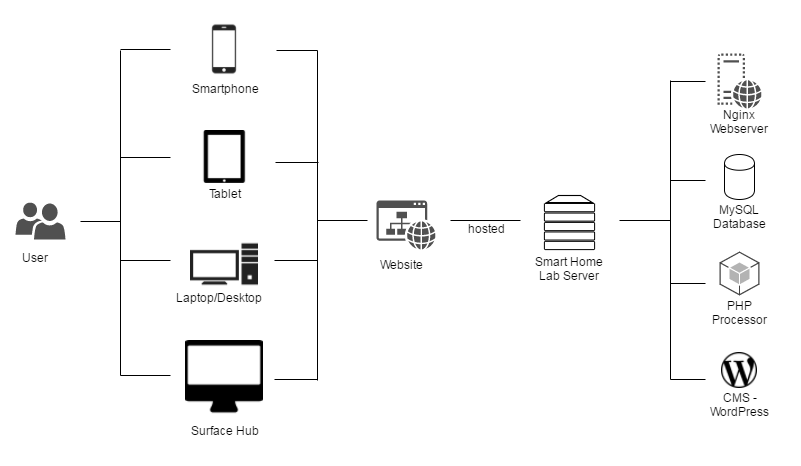
\includegraphics[width=\linewidth,keepaspectratio]{approach/process-diagram.png}
\end{figure}

Figure~\ref{fig:implementation-overview} shows the general implementation of the website for the smart home laboratory. The website is hosted in a physical server, which is located inside the smart home laboratory. This physical server is running the operating system, Ubuntu Server 16.04.2 LTS. In this server, the following software have been installed. They are Nginx HTTP or web server, MySQL database server, PHP application server and WordPress. The website is accessible by using various devices by the users.

\begin{figure}
\caption{The main components of the website}
\label{fig:use-cases-diagram}
\centering
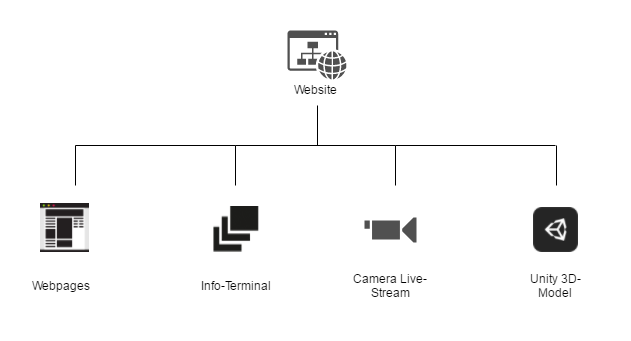
\includegraphics[width=.85\linewidth,keepaspectratio]{approach/use-cases-diagram.png}
\end{figure}

The website in general consists of four parts as shown in the Figure~\ref{fig:use-cases-diagram}. They are:
\begin{description*}
\item[Web pages] represent normal web pages such as Home, About, Components, Panels etc.
\item[Info-Terminal] a full screen web page with slider acts as an automated tour
\item[Live Stream] a web page that has been embedded with live video stream and controllers of an IP Camera
\item[3D-Model] a web page that has been integrated with Unity 3D-Model
\end{description*}

\section{Web Pages}
\subsection*{Header}
Web pages are designed with a header consisting of a main navigation menu. To the left of the main navigation menu, the logo of the institution can be found. To the right of the main navigation menu, a downward arrow can be found. The logo will take user the home page, where else the downward arrow will slide the web page to content part.

\subsection*{Single Column View}
The main body part is programmed to be single-columned view. The reason is to minimize clutters and distractions that can be caused by widgets or banners, and at the same time to give extra focus and emphasize on the main contents.

\subsection*{Sectioning}
The web pages has been separated by sectioning. Each section has been equipped with two arrows -- downward and upward. The idea here is to display a similar group of information in one section. Each section are sized to fit the screen size of HD and FHD screens.

\subsection*{Navigation Arrows}
As mentioned before, each section has two arrows to assist the user to navigate from one section to another. Clicking the upward button will scroll the page automatically to previous section, and clicking the downward button will scroll the web page to next section automatically.

\subsection*{Footer}
An another aspect of the web pages is the footer. The footer as the name itself suggest is to be found at the end of every web page. The footer is divided into two sections. The left section of the footer consists of a copyright statement. The right section of the footer contains a link to \emph{Impressum} page.

\section{Info-Terminal}
\subsection*{Full-Screen Mode}
The info-terminal is programmed to work optimally in full screen mode. It is the only web page, where the header and footer have been removed. The info-terminal consists of only the body part filling the whole screen from left to right and top to bottom.

\subsection*{Screen Ratio}
The info-terminal has been sized to the ratio of 16:9. The reason for choosing the ratio 16:9 is, most of devices' screen are built in this ratio. For example, the Full-HD screen with resolution 1920 x 1080 pixel and HD screen with the resolution 1366 x 768 pixel have this ratio. According to \cite{screen-stat}, this screen ratio counts to more than 50\% of the used devices as of July 2017. It has been found to be wiser and reasonable to choose this screen ratio.

\subsection*{Screen Size}
The screen size of info-terminal is designed with a base resolution of 1920 x 1080 pixel. The reason behind sizing it at this resolution is that the Microsoft Surface Hub has the mentioned resolution. As the info-terminal is targeted to be used mainly with the Surface Hub, it has been sized at this resolution. However, it has been programmed to responsive, which allows it to resize itself accordingly to fit screens of other resolutions.

\subsection*{Autoplay}
The info-terminal slider has been equipped with an autoplay functionality. The autoplay functionality is turned on by default. It is also possible to switch it off, or on, by using the play button located at the top right of the screen.

\subsection*{Navigating}
The info-terminal can be navigated on its own on autoplay mode. Additionally, users can navigate it manually on their own. Here, they can use the left and right arrows which can be found to the left and right edges of the slider respectively. Other than that, the slider can be swiped as well in order to perform the navigation.

\subsection*{Thumbnails}
Thumbnails are one of the feature in the info-terminal. The thumbnails are located at the footer of the slider. Users can see the snipped of the slide on the thumbnails and jump to the slide by clicking it. The thumbnails strip aren't designed with swipe functionality as it conflicts with swipe action on the main slider view.

\subsection*{Home Button}
To the top left of the screen, a home button has been placed. This button will take the user to home page. As the info-terminal doesn't have the header, which contains the main navigation menu, it is essential to provide a button that helps users to navigate back to the home page.

\subsection*{Breadcrumb}
A breadcrumb is the hierarchical navigation link which will be displayed as the user navigate from one level to to another. Breadcrumbs give user a hint on which level they are right now as well as letting them jump to an higher level with a single click.

\subsection*{Location Map}
On the bottom left of the info-terminal, a small lab image has been added. This image displays the location where the components that are being displayed on the current slide can be found in the lab.

\section{Live Stream}
\subsection*{Security Login}
In order to view the live stream of the camera, the web page has been programmed to request the users to provide the IP address, username and password at the beginning. This is to ensure the safety and privacy. Hence, a HTML form has been designed with three fields for each information together with a submit button. Upon submission, the provided information will be validated.

\subsection*{Live Footage}
The live footage has been embedded into HTML multimedia tag. It has been programmed to continuously request for the latest footage from the IP Camera and update the screen as soon as the response footage has been received. The communication happens asynchronously in background.

\subsection*{Controllers}
In addition to viewing the live footage, users also can control the IP camera. For this purpose, nine buttons, each containing an arrow to where the camera should move, have been designed and added to the web page. Using these buttons, users can control the camera in the real time. For each of this button, JavaScript and AJAX programming has been added to communicate with the IP camera.



\chapter{Technologies}
\section{WordPress}
WordPress is one of the famous Content Management System (CMS) that is powering almost 25\% of the websites globally. It is an Open Source project created, developed and maintained by the community. Hence, it can be downloaded, used, modified and distributed freely without any license fees.

The WordPress can be downloaded from their official website, wordpress.org. The current stable version of WordPress is 4.8, as at time of writing. Initially, it started as blogging system and became a full content management system with thousands of plugins, widgets and themes.

To run WordPress, the server should be equipped with PHP version 7 or greater, MySQL database server version 5.6 or greater or MariaDB version 10.0 or greater, and HTTPs support. As for web server, it is recommended to use either Apache or Nginx. They are reliable, have a lot of features, and works well with PHP and MySQL.
For Smart Home Lab website, WordPress will be ran using Nginx web server with PHP and MySQL. The Installation and configuration of them before installing WordPress will be discussed in the next chapter.

With WordPress, various website can be developed right from simple blogs to major websites comprising custom made plugins and widgets. This is one of the advantage of using WordPress is handling the flexibility and complexity while being easy to use.

Using WordPress enables the web developer to concentrate on the contents and structuring the websites, rather than developing the backend and frontend from scratch, which is time consuming and increased time to market.
Other than that, WordPress also provides multilingual pack consisting of 70 languages. This enable the website to developed in multiple languages, primarily in English and German languages. This not only changes the contents of the website as viewed by the web user, but also the administrator dashboard.

WordPress also provides excellent security for its users. Their security implementation consists of protection against Injection, Broken Authentication, Cross Site Scripting (XSS), Insecure Direct Object Reference, Security Misconfiguration etc. Their themes, plugins as well as hosting providers are tested and secured.

Using WordPress also make it easy for others to develop and continue the development of the website in the future, as everything can be managed in an easy web interface. And through this documentation, most of the essential information regarding the installation, configuration and contents development will be provided.

\section{PHP}
PHP stands for Hypertext Preprocessor. It is a general-purpose scripting language for generating dynamic web contents. It is commonly used for web development and can be embedded into HTML. The PHP scripts are executed on the server-side and the clients are unaware of the script and its execution. The result of the executed PHP will be sent to client in HTML format.

PHP scripts are processed by PHP parser or PHP interpreter. This parser will be installed in the web server such as Apache, IIC, lighttpd or Nginx as a Common Gateway Interface (CGI). The PHP parser is open source software, which can be downloaded from their official website\footnote{http://php.net}.

PHP is not only limited to deliver web contents like HTML, but can be used to output text, images, PDFs and flash-videos. One of the PHP advantages is it supports and works well with various databases. For this website, the database called MySQL is used and will be discussed in the next section.

\section{MySQL}
MySQL is relational database management system (RDBMS). The Community Edition of MySQL is open source database system which can be downloaded from the official website\footnote{https://dev.mysql.com/downloads/}. MySQL uses structured query language (SQL) to query, filter, add, modify and delete data in the database. The data in the database will be arranged in table form. MySQL is used in majority of the websites and content management system such as WordPress.

\section{Nginx}
Nginx is a high-performance web server. It is also act as reverse proxy, IMAP/POP3 proxy server, load balancer and accelerator. It works with HTTP-, TCP- as well as UDP-based services. The main advantages of Nginx are its high performance, stability, rich feature set, simple configuration and low resource consumption.

The architecture of Nginx uses scalable event-drive asynchronous architecture. Not only it uses small amount of memory, but the memory usage is predictable under load. It success relies in the ability to handle thousands of requests at the same time. For this project, Nginx web server will be used, where it communicates with PHP parser to run WordPress and MySQL database.


\chapter{Server Setup and WordPress Installation}

In this project, WordPress is setup on Nginx HTTP web server running PHP preprocessor and MySQL database server. This chapter will explain on how to configure Ubuntu server, setup Nginx, PHP, MySQL database as well as WordPress.

\section{Ubuntu Server Configuration} \label{sec:ubuntu-server-configuration}
The Smart Home Lab has its own server running Ubuntu Server 16.04.2 LTS. On this server, a \ac{vm} application has been installed. This VM runs a separate virtual Ubuntu Server on the host. This VM has been allocated with its own processing power, memory and disk space. Local machine can connect to the virtual Ubuntu Server using the Wi-Fi network, SHLAB02 as shown in Figure~\ref{fig:shlab02-wlan-network}.

\begin{figure}[ht]
\caption{SHLAB02 WLAN network to connect to Ubuntu Server}
\label{fig:shlab02-wlan-network}
\centering
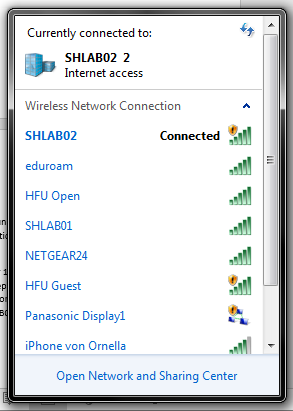
\includegraphics[height=5cm,keepaspectratio]{setup/shlab02-wlan-network.png}
\end{figure}

On the local machine, first, a \ac{ssh} key or commonly known as public/private key should be generated. This can be done using the PuTTY Key Generator application as shown in Figure~\ref{fig:putty-key-generator}. This application can be downloaded at the URL given in the footnote\footnote{http://www.chiark.greenend.org.uk/~sgtatham/putty/latest.html}. The current stable version of Putty Key Generator is 0.68, as at time of writing.

\begin{figure}[ht]
	\begin{subfigure}{.49\linewidth}
	\caption{PuTTY SSH Key Generator}
	\label{fig:putty-key-generator}
	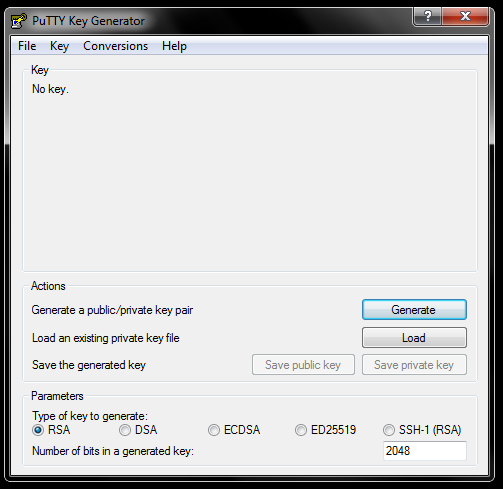
\includegraphics[width=\textwidth,keepaspectratio]{setup/putty-key-generator.png}
	\end{subfigure}
	\begin{subfigure}{.49\linewidth}
	\caption{Generating random key in PuTTY}
	\label{fig:putty-random-key}
	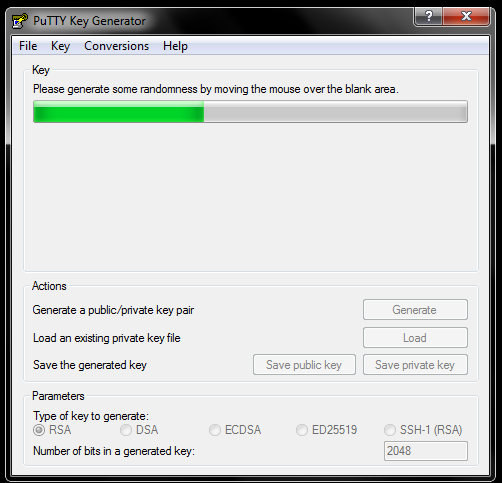
\includegraphics[width=\textwidth,keepaspectratio]{setup/putty-random-key.png}
	\end{subfigure}
\end{figure}

The keys can be generated by clicking generate button and by moving the mouse cursor randomly at the blank area as shown in Figure~\ref{fig:putty-random-key}. After that, the Key Passphrase and Confirm Passphrase must be given. This Passphrase must be noted down or remembered for future usage when connecting to the server every time. The Passphrase is \texttt{BSY2qjtu\$\#}

The generated Public Key and Private Key must be saved. The generated Public Key will be provided to the virtual Ubuntu Server running on the server. Where else the generated Private Key must be saved in the local machine that will be used to connect to the server.

\begin{figure}[ht]
\centering
	\begin{subfigure}{.49\linewidth}
	\caption{Host Name and Port}
	\label{fig:putty-connect}
	\centering
	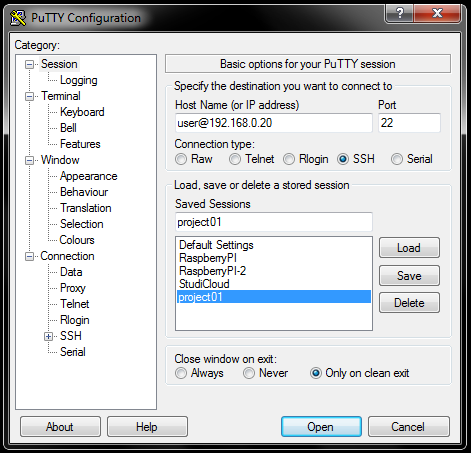
\includegraphics[width=\textwidth,keepaspectratio]{setup/putty-connect.png}
	\end{subfigure}
	\begin{subfigure}{.49\linewidth}
	\caption{Attaching Private Key}
	\label{fig:putty-private-key}
	\centering
	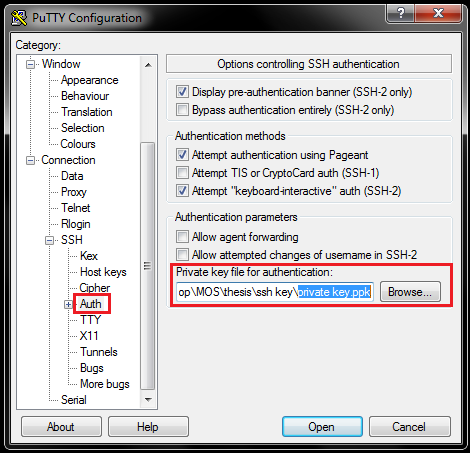
\includegraphics[width=\textwidth,keepaspectratio]{setup/putty-private-key.png}
	\end{subfigure}
\end{figure}

To connect to the server, the PuTTY application will be used. This application can be downloaded at the same link as the PuTTY Key Generator link given above. The PuTTY application will be provided with Host Name (or IP Address) of the server, which is \texttt{user@192.168.0.20} and Port number, which is\texttt{ 22} as shown in the Figure~\ref{fig:putty-connect}. After that the generated Private Key from previous step must be given in the ‘Private key file for authentication’ field as shown in Figure~\ref{fig:putty-private-key}. This field can be found under Connection > SSH > Authentication tab. Lastly ‘X11 forwarding’ must be enabled. Connection to the server can be established by pressing ‘Open’ button.

After successfully connecting, the passphrase, \texttt{BSY2qjtu\$\#} that have been entered while generating the Public/Private keys must be entered in the terminal to proceed.

\section{Nginx HTTP Server Installation} \label{sec:nginx-http-server-installation}
Nginx is a powerful, versatile and efficient HTTP or web server. Nginx web server can be installed in Ubuntu using the \texttt{apt} package.

\subsection{Step 1: Installing Nginx}
The following has been used to install Nginx.
\begin{lstlisting}
$  sudo apt-get update
$  sudo apt-get install nginx
\end{lstlisting}

\subsection{Step 2: Enabling Nginx}
The Ngnx, by default, will be configured and started running automatically after the installation. If the server runs firewall, the Nginx should be enabled manually. The Nginx will however register itself with the server firewall, which is \texttt{ufw} upon installation. The following command has to be ran in the terminal to start the Nginx manually.

\begin{lstlisting}
$  sudo ufw allow 'Nginx HTTP'
\end{lstlisting}

\subsection{Step 3: Checking Nginx Status}
The status of Nginx HTTP server can be checked by using the following command.

\begin{lstlisting}
$  sudo ufw status
\end{lstlisting}

Running this command will output the following.
\begin{table}[ht]
\begin{tabular}{l l l}
To & Action & From \\
-- & -- & -- \\
OpenSSH & ALLOW & Anywhere \\
Nginx HTTP & ALLOW & Anywhere \\
OpenSSH  (v6) & ALLOW & Anywhere \\
Nginx HTTP (v6) & ALLOW & Anywhere \\
\end{tabular}
\end{table}

The output on the second and third column which are 'ALLOW' and 'Anywhere' respectively indicates that the Nginx is running. The successful installation of Nginx can be further tested using any web browser by entering the host's IP address, which in this case \texttt{http://192.168.0.20}. The following page will be displayed as shown in the Figure~\ref{fig:nginx-start-screen}.

\begin{figure}[ht]
\caption{Nginx Default Start Screen}
\label{fig:nginx-start-screen}
\centering

\includegraphics[height=5cm,keepaspectratio]{setup/nginx-start-screen.png}
\end{figure}


\section{MySQL Database Installation} \label{sec:mysql-database-installation}
After installing Nginx HTTP server, database server has been installed to manage the storing of the website content. In this project MySQL database server has been used.

\subsection{Step 1: Installing MySQL}
The following command has to be entered to install MySQL database on the Ubuntu server. 
\begin{lstlisting}
$  sudo apt-get install mysql-server
\end{lstlisting}

During the installation, root password will be prompted or asked. Here, the password \texttt{d\_XKdEoCwX,4EnO} has been given. Here are the MySQL database credentials for future reference:
\begin{itemize*}
\item username: root
\item password: d\_XKdEoCwX,4EnO
\end{itemize*}

\subsection{Step 2: Securing MySQL Database}
This section will discuss on how to secure the MySQL database server. To get started, the following command has to be entered in the terminal.
\begin{lstlisting}
$  sudo mysql_secure_installation
\end{lstlisting}

Running this command will take us through security setup of MySQL database server which consist of a series of questions. Here are the three questions and the settings that have been given for the future reference. The rest of settings have been given 'yes' as the answers.

\begin{lstlisting}
VALIDATE PASSWORD PLUGIN can be used to test passwords
and improve security. It checks the strength of password
and allows the users to set only those passwords which are
secure enough. Would you like to setup VALIDATE PASSWORD plugin?

Press y|Y for Yes, any other key for No: y


There are three levels of password validation policy:
LOW    Length >= 8
MEDIUM Length >= 8, numeric, mixed case, and special characters
STRONG Length >= 8, numeric, mixed case, special characters and dictionary file

Please enter 0 = LOW, 1 = MEDIUM and 2 = STRONG: 1


Using existing password for root.

Estimated strength of the password: 100
Change the password for root ? ((Press y|Y for Yes, any other key for No) : n
\end{lstlisting}

\section{PHP Preprocessor Installation} \label{sec:php-preprocessor-installation}
Nginx web server does not contain native PHP preprocessor. A package called \texttt{php-fhm}, which stand for "fastCGI process manager" must be installed on the Ubuntu server. This package tells Nginx to pass the PHP request to \texttt{php-fhm} for processing. Second package that has to be installed is \texttt{php-mysql}, which allows PHP to communicate with the database server.

\subsection{Installing php-fpm and php-mysql}
The following command has been entered to install \texttt{php-fpm} and \texttt{php-mysql}.
\begin{lstlisting}
$  sudo apt-get install php-fpm php-mysql
\end{lstlisting}

\subsection{Securing PHP configuration}
Initial installation of PHP has to be secured by commenting out the \texttt{cgi\_fix\_pathinfo} line and setting its value to \texttt{0} in the PHP configuration file, \texttt{php.ini}.

\begin{lstlisting}
$  sudo nano /etc/php/7,0/fpm/php.ini

/etc/php/7.0/fpm/php.ini
...
cgi\_fix\_pathinfo=0
...
\end{lstlisting}

Save and close the nano editor. Next, the PHP preprocessor has to be restarted so that the changes will take effect by entering the following command.

\begin{lstlisting}
$  sudo systemctl restart php7.0-fpm
\end{lstlisting}

\subsection{Configuring Nginx to use PHP Preprocessor}
In this section, a few settings changes on the Nginx will be shown in order to ask Nginx to use PHP preprocessor. The server settings of Nginx can be opened using the following command.

\begin{lstlisting}
$  sudo nano /etc/nginx/sites-available/default
\end{lstlisting}

After opening the server settings, \texttt{index.php} has to be added to index line in the server block. In addition to that, two new block \texttt{location \~\textbackslash php\$} and \texttt{location \~/\textbackslash .ht \{} has to be introduced.

\begin{lstlisting}
server {
    ...
    index index.php

    location ~ \.php$ {
        include snippets/fastcgi-php.conf;
        fastcgi_pass unix:/run/php/php7.0-fpm.sock;
    }

    location ~ /\.ht {
        deny all;
    }
}
\end{lstlisting}

After adding those lines to the Nginx configuration files, the configuration file has to be checked for error. If no error is reported, the web server can be restarted safely as shown below.

\begin{lstlisting}
$  sudo nginx -t
$  sudo systemctl reload nginx
\end{lstlisting}

\subsection{Testing PHP Preprocessor}
The installation and configuration of PHP preprocessor can be tested by introducing \texttt{info.php} to the server root directory. A PHP information file can be created by using the following command.

\begin{lstlisting}
$  sudo nano /var/www/html/info.php
\end{lstlisting}

In the PHP file, following lines have to be added. After adding those lines, save and close the file.
\begin{lstlisting}
<?php
    phpinfo();
\end{lstlisting}

Now the PHP preprocessor can be tested using web browser by entering the URL, \texttt{http://192.168.0.20/info.php}. After testing the PHP preprocessor, it is important that \texttt{info.php} file has to be deleted to prevent anyone from learning the PHP configurations.

\section{WordPress Installation} \label{sec:wordpress-installation}
After installing Nginx, PHP and MySQL, we can begin with WordPress installation. Please make sure to log in into server-side using PuTTY. Before we can install the WordPress, there are few settings / configurations that have to be done, which includes:
\begin{itemize*}
\item Setting up database table and database user
\item Configuring Nginx server
\item Installing additional PHP modules to handle WordPress
\item Generating secret keys
\item Downloading latest stable version of WordPress
\item Configuring WordPress
\end{itemize*}

\subsection*{Step 1: Creating MySQL Database and User}

First, we need to prepare a database table and user in the installed MySQL. The database table and user will then be used by WordPress to store data and access them.

Start MySQL database by issuing the following command:

\begin{lstlisting}
$ mysql -u root -p
\end{lstlisting}

Enter the password \texttt{d\_XKdEoCwX,4EnO} for the user \texttt{root} when prompted.

Create a new database table \texttt{wordpress} by issuing following command. And don't forget the semicolon at the end of the line.
\begin{lstlisting}
mysql > CREATE DATABASE wordpress DEFAULT CHARACTER SET utf8 COLLATE utf8_unicode_ci;
\end{lstlisting}

Next, create a new user to operate the above created \texttt{wordpress} database. The following command will create a new user \texttt{wordpressuser} with password \texttt{ABcd1234\#}.

\begin{lstlisting}
myql > GRANT ALL ON wordpress.* TO 'wordpressuser'@'localhost' IDENTIFIED BY 'ABcd1234#';
\end{lstlisting}

This will create the new user with given password, as well as granting the user the all accesses to the database \texttt{wordpress}. Finally, flush the privileges so that the MySQL aware of the changes we have made and exit MySQL.

\begin{lstlisting}
mysql > FLUSH PRIVILEGES;
mysql > EXIT;
\end{lstlisting}


\subsubsection*{Step 2: Adjust Nginx's Configuration}
There are two modifications that have to be made to the Nginx web server to handle WordPress correctly:
\begin{enumerate}
\item Instruct server not to log requests for the static files with extensions such as .css, .gif etc.
\item Insert \texttt{index.php} into \texttt{try\_files}
\end{enumerate}

Open the Nginx configuration file using \texttt{sudo} privileges:
\begin{lstlisting}
$ sudo nano /etc/nginx/sites-available/default
\end{lstlisting}

We can request server not to log requests to the static files by issuing command {\tt log\_not\_found off}. It is a best practice not to log requests to static files.

\begin{lstlisting}
server {
	...
	location = /favicon.ico {
		log_not_found off;
		access_log off
	}
	location = /robot.txt {
		log_not_found off;
		access_log off;
		allow all;
	}
	location ~* \.(css|gif|ico|jpeg|jpg|js|png)$ {
		expires max;
		log_not_found off;
	}
	...
}
\end{lstlisting}

For the second task, passing \texttt{index.php} as \texttt{try\_files} is done so that the server will return home page instead of 404 error as a default option. To do this, following line has to put inside \texttt{location /} block.

\begin{lstlisting}
server {
	...
	location / {
		#try_files $uri $uri/ =404;
		try_files $uri $uri/ /index.php$is_args$args;
	}
	...
}
\end{lstlisting}

When these changes have been made, save the configuration file and exit \texttt{nano} editor by pressing \texttt{Ctrl-x}. Check for the syntax errors of the new configurations. If no error is been reported, restart the Nginx.

\begin{lstlisting}
$ sudo nginx -t
$ sudo systemctl reload nginx
\end{lstlisting}

\subsubsection*{Step 3: Installing additional PHP extensions}
PHP preprocessor has been installed and setup with minimal setting in the previous section. Here, additional modules or extensions will be installed, which is required by WordPress \cite{SugarHill.2016}. Use to following command to install the required additional extensions:

\begin{lstlisting}
$ sudo apt-get update
$ sudo apt-get install php-curl php-gd php-mbstring php-mcrypt php-xml php-xmlrpc
\end{lstlisting}

After finish installing the extensions, restart the \texttt{php-fpm} process.
\begin{lstlisting}
$ sudo systemctl restart php7.0-fpm
\end{lstlisting}

\subsubsection*{Step 4: Generating secret keys}
Secret keys have to be generated to provide security for the WordPress. The secret keys are provided by WordPress through their secure key generator. To get secret keys from WordPress key generator, issue the following command on the terminal:

\begin{lstlisting}
$ curl -s https://api.wordpress.org/secret-key/1.1/salt
\end{lstlisting}

Or another workaround is to use the web browser. Enter the URL \texttt{https://api.wordpress.org/secret-key/1.1/salt} and press enter. Save the generated secret keys, which must be used in the next step.


\subsubsection*{Step 5: Downloading WordPress}
Download the latest version of stable WordPress from https://wordpress.org website. After downloading, extract the downloaded content.

\begin{lstlisting}
$ cd /tmp
$ curl -o https://wordpress.org/latest.tar.gz
$ tar xzvf latest.tar.gz
\end{lstlisting}

By default, WordPress has provided a sample copy of the WordPress configuration file. This file can be found under directory and file name \texttt{tmp/wordpress/wp-config-sample.php}.

Copy the provided configuration file to used in our website. And Create a new directory \texttt{upgrade}, so that WordPress can upgrade its software in the future without any permission issue.
\begin{lstlisting}
$ cp /tmp/wordpress/wp-config-sample.php /tmp/wordpress/wp-config.php
$ mkdir /tmp/wordpress/wp-content/upgrade
\end{lstlisting}

Finally, copy the contents into root server directory. This are the contents used by the Nginx web server to serve when request is made to the website.
\begin{lstlisting}
$ sudo cp -a /tmp/wordpress/. /var/www/html
\end{lstlisting}

\subsubsection*{Step 6: Configuring WordPress}
Open the WordPress configuration file:
\begin{lstlisting}
$ nano /var/www/html/wp-config.php
\end{lstlisting}

In the file, find the 'secret key' section, which appears as follow and paste the generated secret keys from Step 4.
\begin{lstlisting}
...
define('AUTH_KEY', 'put your unique phrase here');
define('SECURE_AUTH_KEY', 'put your unique phrase here');
define('LOGGED_IN_KEY', 'put your unique phrase here');
define('NONCE_KEY', 'put your unique phrase here');
define('AUTH_SALT', 'put your unique phrase here');
define('SECURE_AUTH_SALT', 'put your unique phrase here');
define('LOGGED_IN_SALT', 'put your unique phrase here');
define('NONCE_SALT', 'put your unique phrase here');
...
\end{lstlisting}


After pasting the generated secret keys, the MySQL database credentials have to be given. These credentials have been created in the Step 1.
\begin{lstlisting}
...
define('DB_NAME', 'wordpress');

/** MySQL database username */
define('DB_USER', 'wordpressuser');

/** MySQL database password */
define('DB_PASSWORD', 'ABcd1234#');
\end{lstlisting}

Lastly, we need to give permission to Nginx web server to write where it needs to. Otherwise, WordPress will be asking FTP credentials when any actions need to be performed. This can be done through following setting:
\begin{lstlisting}
define('FS_METHOD', 'direct');
\end{lstlisting}

Save the \texttt{wp-config.php} file and exit the nano editor.

\subsubsection*{Step 7: Complete WordPress Installation}
We need to complete the WordPress installation now through the web browser. Open the web browser and enter the URL \texttt{192.168.0.20}. First, we need to select the language.

\begin{figure}[ht]
\caption{WordPress language selection}
\label{fig:wordpress-language-selection}
\centering
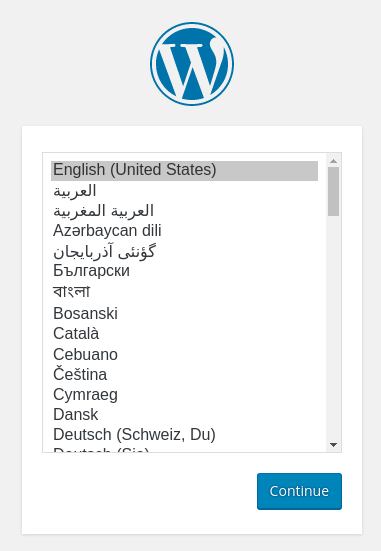
\includegraphics[height=5cm,keepaspectratio]{setup/language-selection.png}
\end{figure}

After that, we need to provide a few information on the main setup page such as \emph{Site Title}, \emph{Username}, \emph{Password} and \emph{Email}.

\begin{figure}[ht]
\caption{Main WordPress setup page}
\centering
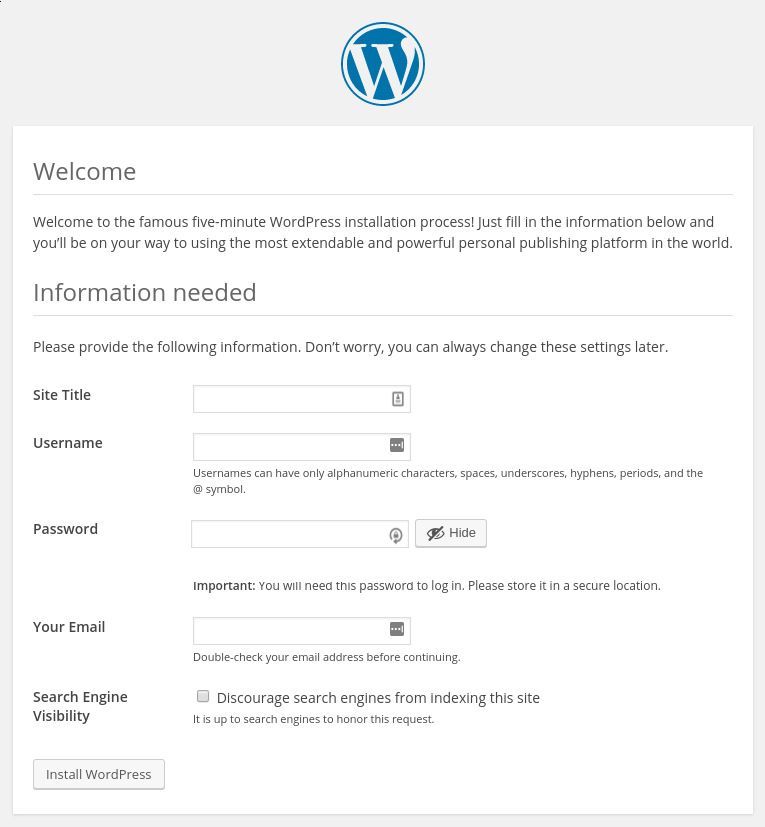
\includegraphics[height=6cm,keepaspectratio]{setup/main-wp-setup.png}
\end{figure}

These are information given on the page shown above:
\begin{itemize*}
\item Site Title: Smart Home Lab
\item Username: ashiqmoh
\item Password: oSm0cCCAguIMsalrZd(\#2i5(
\item Email: ashiqmoh@192.168.0.20
\end{itemize*}

The installation can be completed by clicking 'Install WordPress' button. Upon installation, the administration side of the website can be accessed by entering following URL:
\begin{lstlisting}
http://192.168.0.20/wp-admin
\end{lstlisting}

Provide the username and password stated above and login. The administration side of the website appears as shown in the figure below.

\begin{figure}[ht]
\caption{Administation page of WordPress}
\centering
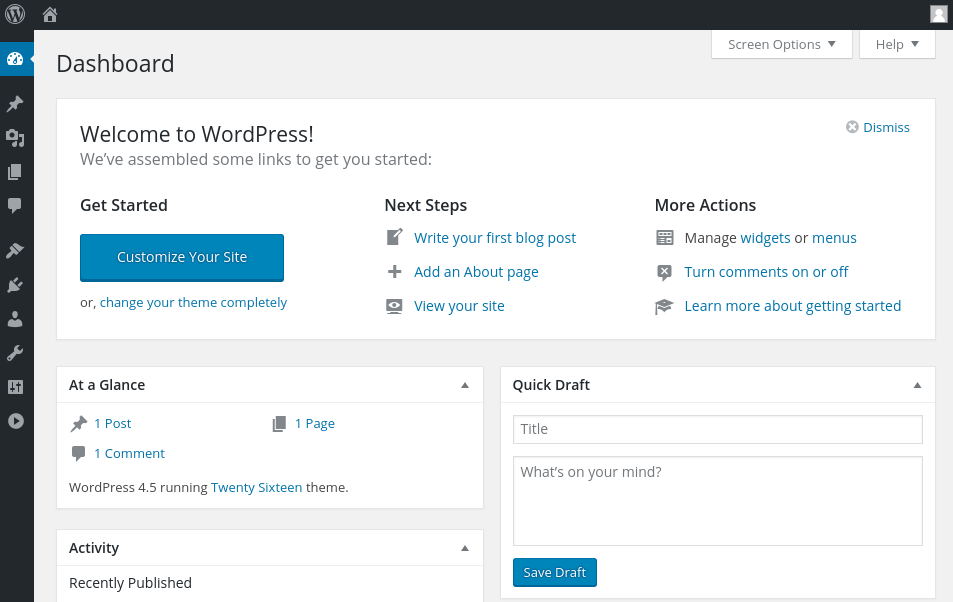
\includegraphics[height=7cm,keepaspectratio]{setup/wp-admin-page.png}
\end{figure}

\section{Routing WordPress to external URL} \label{sec:routing-wordpress-to-external-url}
The website i.e. WordPress, that has been installed inside one of the virtual machine in the Smart Home Lab physical server, by default can be accessed internally only through the \ac{ip} address \texttt{192.168.0.20}. To make the website accessible from external network through an \ac{url} address, the following steps have to be done.

Go to the general settings of the WordPress by clicking \scalerel*{
\includegraphics{setup/settings-button.png}}{B} button from the left navigation menus. Then, click on the \scalerel*{
\includegraphics{setup/general-button.png}}{B} button from the sub-menus.

Here, the following fields can be changed from \texttt{192.168.0.20} to the desired \ac{url} address:
\begin{itemize*}
\item WordPress Address (URL)
\item Site Address (URL)
\end{itemize*}

Both the text fields have been changed to the URL address:
\begin{lstlisting}
http://web.smarthome.hs-furtwangen.de
\end{lstlisting}

By doing this, the website can be accessed externally.

\section{Restrict Website Access to Internal Network}
The access to the website from external network can be revoked and restrict it to be accessible only from within the lab network by reversing the process described in the Section~\ref{sec:routing-wordpress-to-external-url}. The \emph{WordPress Address (URL)} and \emph{Site Address (URL)} text fields have to be changed to the \ac{ip} address \texttt{192.168.0.20}.



\chapter{Website Designing}
The Smart Home Lab website consists of 5 web pages. Those are:
\begin{itemize*}
\item Home
\item The Lab
\item Components
\item Panels
\item Use Cases
\end{itemize*}

These web pages have been created and designed within the WordPress by using a WordPress plugin called 'Page Builder By SiteOrigin'. This chapter will discuss on how these web pages has been created and designed, as well as the important steps and settings involved in it.

\section{Enabling Page Builder Plugin}
Firstly, the 'Page Builder by SiteOrigin' has to be downloaded and activated in the WordPress. This can be done through the 'Plugins' section in the admin side of the WordPress. After downloading and activating the plugin, the Page Builder plugin will automatically add a tab on the top right of the page editor (refer Figure~\ref{enabling-page-builder}), when a new page has been created. The usage of Page Builder can be enabled simply by clicking on this tab.

\begin{figure}[ht]
\centering
\caption{Enabling Page Builder Plugin}
\label{enabling-page-builder}
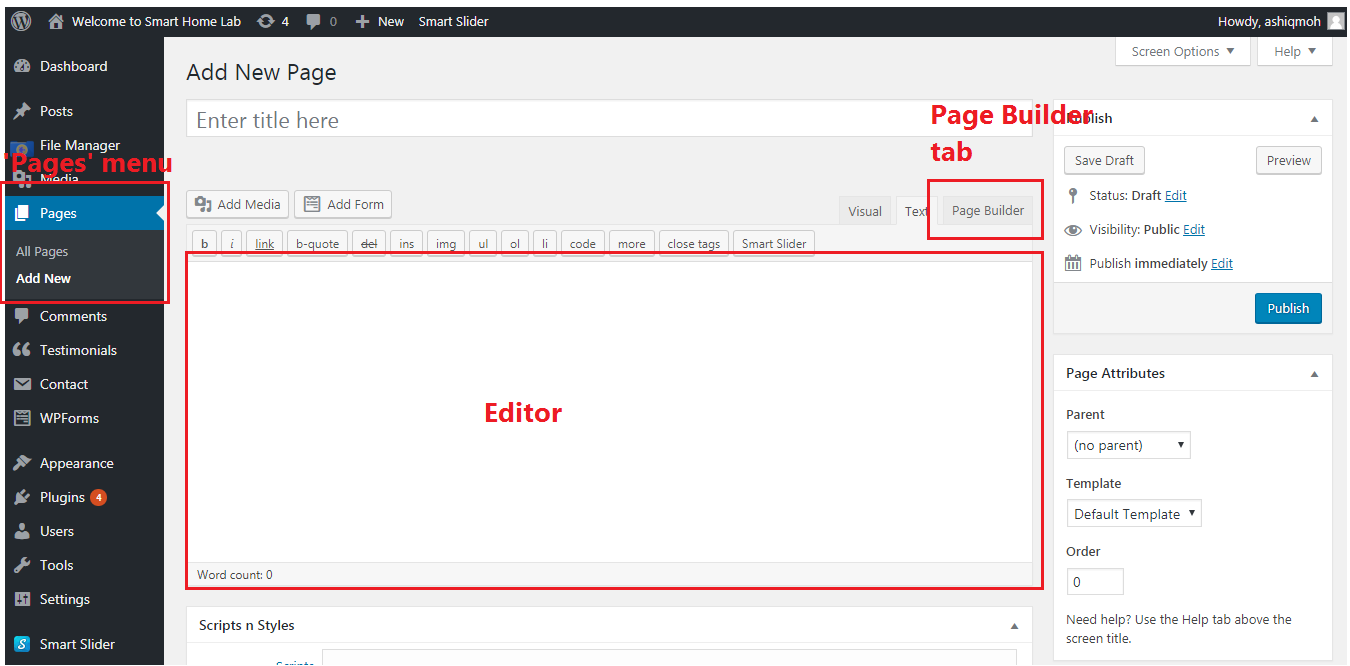
\includegraphics[height=5cm,keepaspectratio]{website-designing/enabling-page-builder.png}
\end{figure}

\section{Adding row, column and widget}
When Page Builder plugin has been enabled, the editor will display a series of buttons on the top of the editor. One of the important thing here is the 'Add Row' option. A row in the page builder signifies a horizontal section in a web page as shown in the Figure~\ref{row-section-explanation}. Each of this section is a row.

\begin{figure}[ht]
\centering
\caption{A row representing a horizontal column on the website}
\label{row-section-explanation}
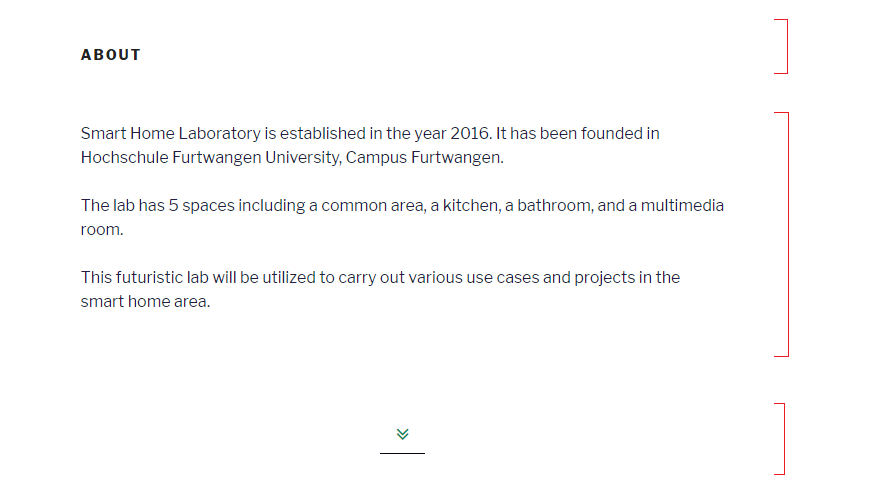
\includegraphics[height=5cm,keepaspectratio]{website-designing/row-section-explanation.png}
\end{figure}

When the 'Add Row' button (see~Figure \ref{adding-row}) is clicked, a new window (see Figure~\ref{adding-column}) will be opened asking to set the column. Here, the number of columns as well as the individual size of the column has to be given in.

\begin{figure}[ht]
\centering
	\begin{subfigure}{.49\linewidth}
	\centering
	\caption{Adding Row}
	\label{adding-row}
	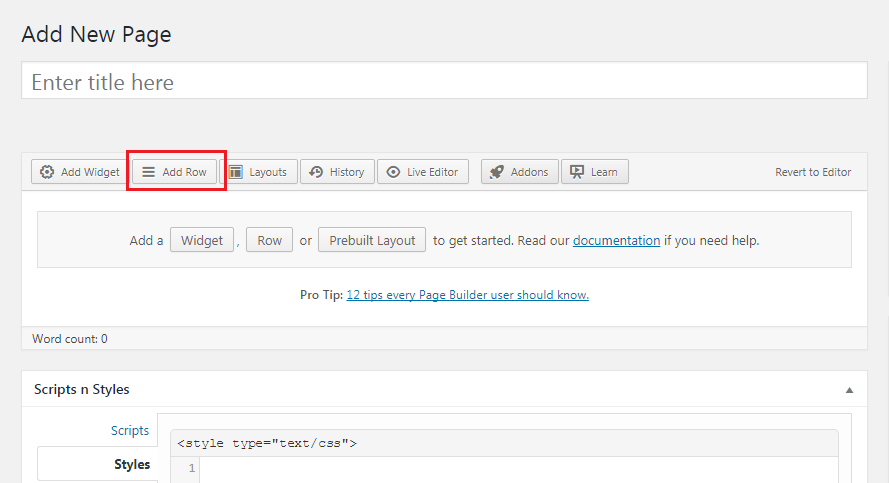
\includegraphics[width=\textwidth,keepaspectratio]{website-designing/adding-row.png}
	\end{subfigure}
	\begin{subfigure}{0.49\linewidth}
	\centering
	\caption{Adding Column}
	\label{adding-column}
	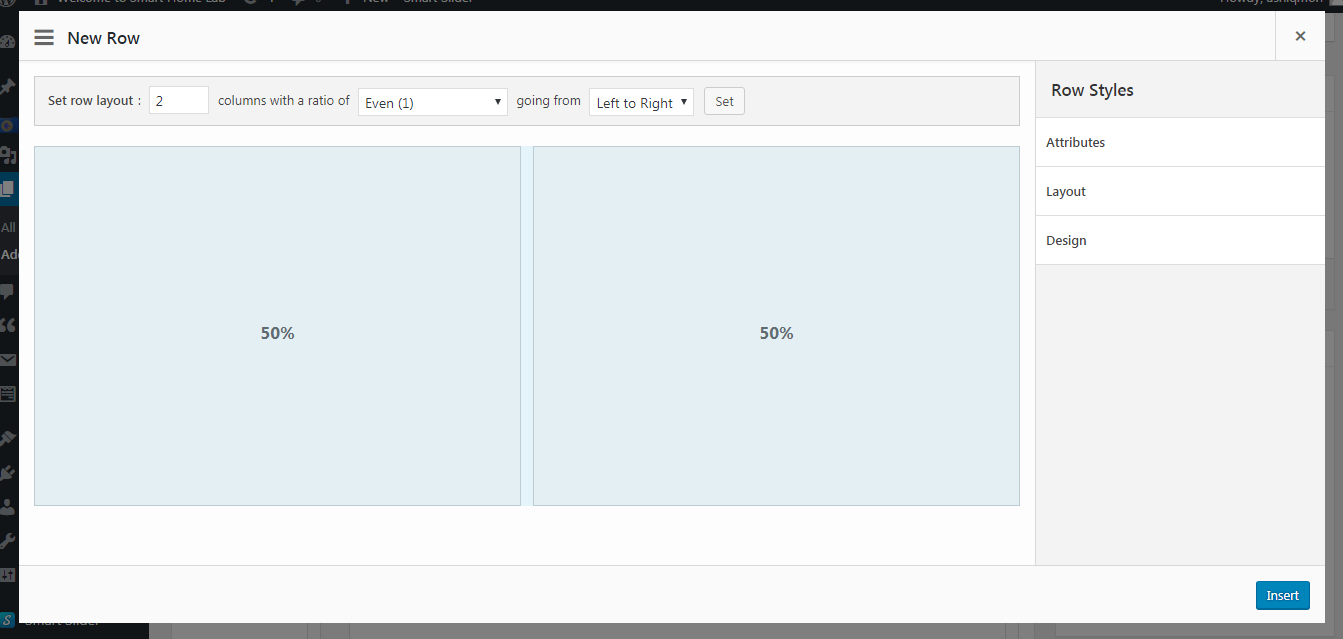
\includegraphics[width=\textwidth,,keepaspectratio]{website-designing/adding-column.png}
	\end{subfigure}
\end{figure}

After a row and a column (optionally multiple columns to a row) have been added, the editor will display a box within it. Within this box, widgets can be added by clicking the 'Add Widget' button next to the 'Add Row' button. When this button is clicked, a new window (see Figure~\ref{list-of-widgets} will pop up prompting which widget to be added into the created row i.e. column. The list of widgets consists of, for an example, 'SiteOrigin Editor', 'SiteOrigin Button', 'SiteOrigin Button' etc. To add normal text into the web page, one need to insert the 'SiteOrigin Editor' widget into the row. For a short note, multiple widgets can be inserted into a single row i.e. column.

\begin{figure}[ht]
\centering
\caption{Window showing a list of widgets to be inserted in to row i.e. column}
\label{list-of-widgets}
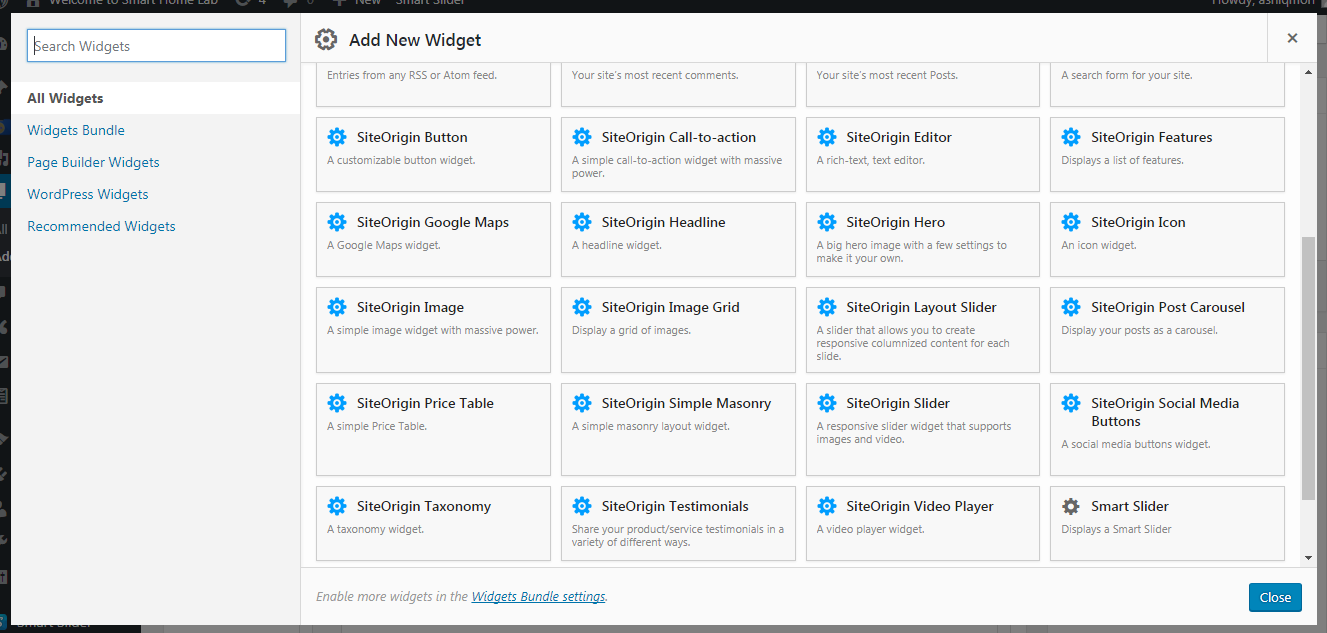
\includegraphics[height=5cm,keepaspectratio]{website-designing/list-of-widgets.png}
\end{figure}

Here is an example of screenshot of page builder row before and after adding a widget. In this example, the SiteOrigin Editor widget has been added.

\begin{figure}[ht]
\centering
	\begin{subfigure}{.49\linewidth}
	\centering
	\caption{Row before adding widget}
	\label{row-before-adding-widget}
	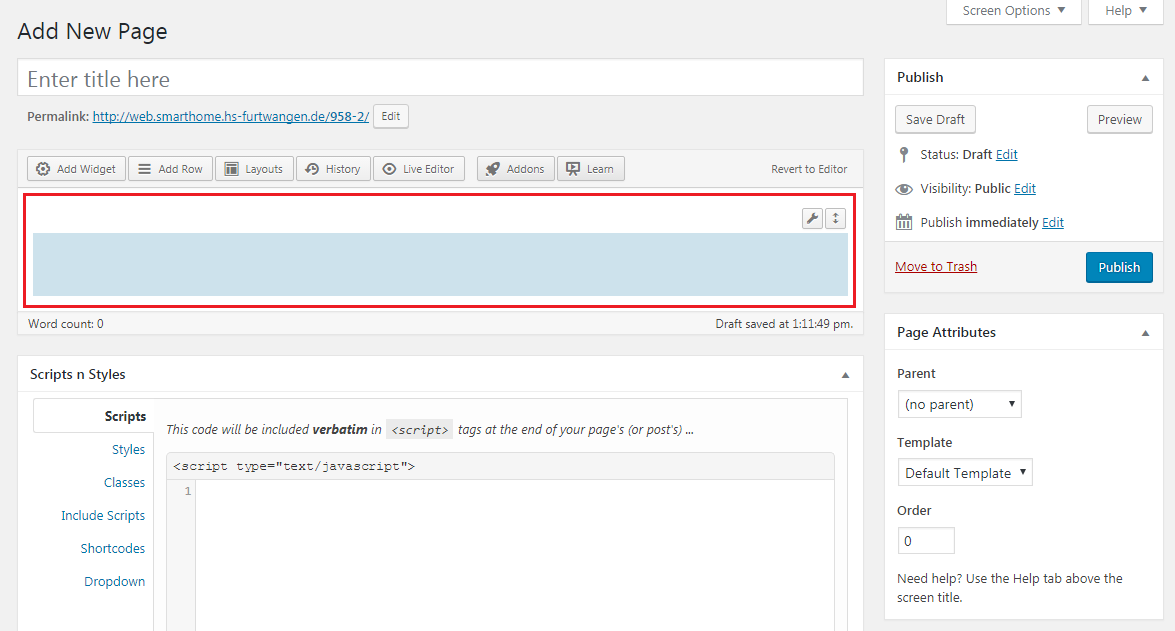
\includegraphics[width=\textwidth,keepaspectratio]{website-designing/row-before-adding-widget.png}
	\end{subfigure}
	\begin{subfigure}{0.49\linewidth}
	\centering
	\caption{Row after adding widget}
	\label{Row after adding widget}
	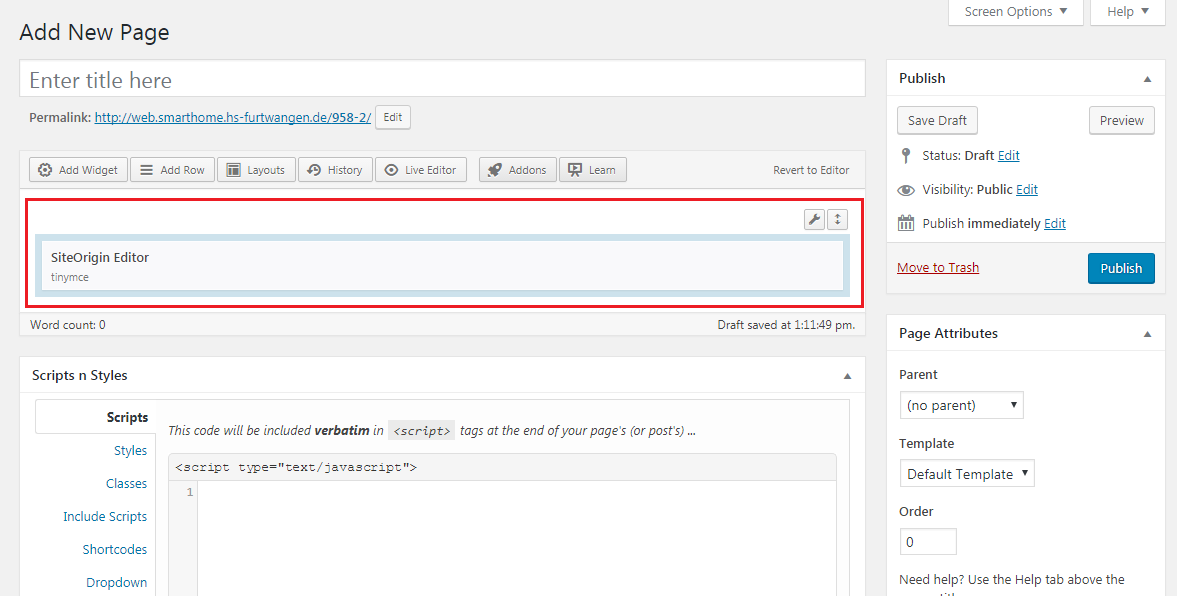
\includegraphics[width=\textwidth,,keepaspectratio]{website-designing/row-after-adding-widget.png}
	\end{subfigure}
\end{figure}

\section{Adding text, image and button}
Text can be added into the web page through the SiteOrigin Editor plugin. After the SiteOrigin Editor plugin has been inserted into the row/column, a menu list will appear when one hover the mouse over it. In the menu list, the 'edit' option has to be clicked to open the editor. In the editor, the text that has been intended to be added to web page can be typed. Text here can represent the header text and the normal paragraph text.

Next, in order to add an image, the SiteOrigin Image plugin can be used. After inserting the plugin, throught the edit option, a new window will be opened. Here, the URL of image as well as other settings such as image size, image alignment, image title etc. can be entered.

The button which are found on the web pages are added through the SiteOrigin Button plugin. Same as step above, after adding the plugin, one has to click on the 'edit' option on mouse over. Here, one has to define the destination URL which will be opened when the button is clicked. Optionally, the text or icon that should appear on the button can be added. There are also other options for alignment layout designing of the button.

\section{Adding Scroll Effect}
As can be noticed, clicking on the button scroll the content to a specific part of the web page. To enable the scroll effect, a few steps have to be taken.

First, a plugin called 'Page Scroll to Id' has to be added and activated in the WordPress. After adding and activating, buttons that have been added has to be given the class name 'ps2id'. The class name of a button can be given by the 'edit' option mentioned in the previous section. In the edit section, under the 'Other attributes and SEO', the class name can be given in the 'Button Classes' field as can be seen in the Figure~\ref{button-class-name}.

\begin{figure}[ht]
\centering
\caption{Button Classes field where 'ps2id' has to be entered}
\label{button-class-name}
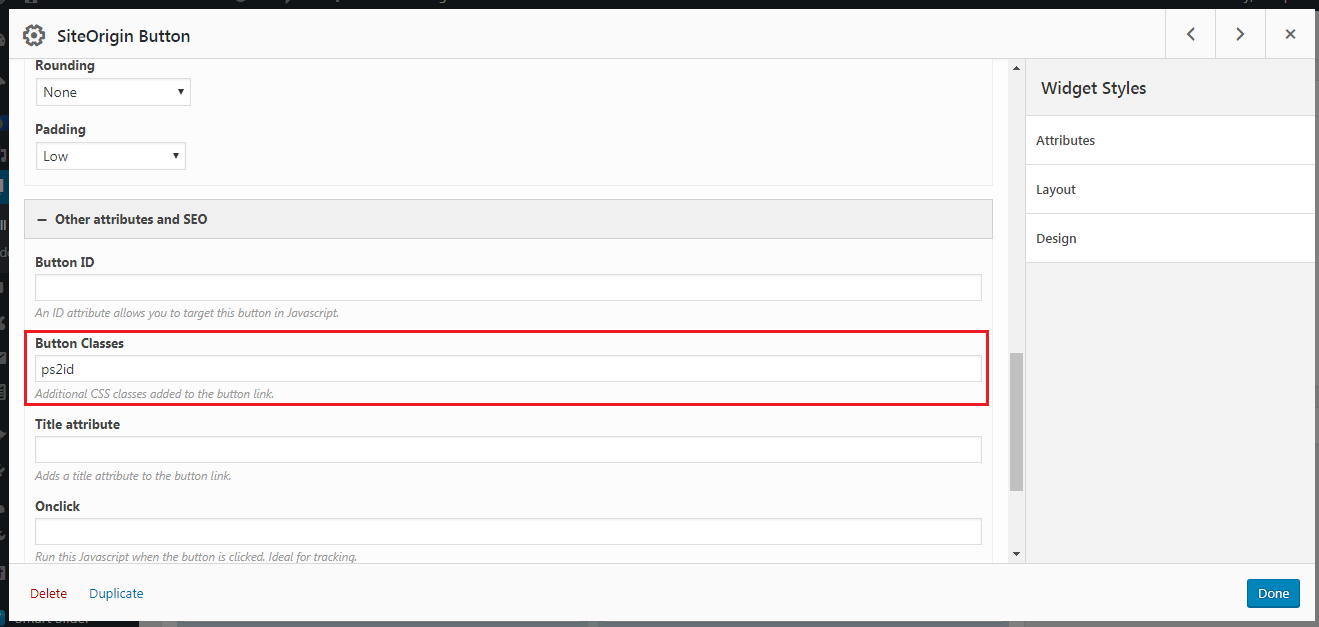
\includegraphics[height=5cm,keepaspectratio]{website-designing/button-class-name.png}
\end{figure}

Lastly, the destination URL has to be set. The destination \ac{url} has to be entered in two places. First in button edit section, under the 'Destination URL' field as can be seen in the Figure~\ref{destination-url-button}.  Secondly, the same destination URL has to be given to 'Row ID' field of the target element. The step to provide the target element an id is shown in the Figure~\ref{target-element-id}. By assigning the button and the target element the id, the button will scroll the web page to target element.

\begin{figure}[ht]
\centering
\caption{Adding the destination URL for a button}
\label{destination-url-button}
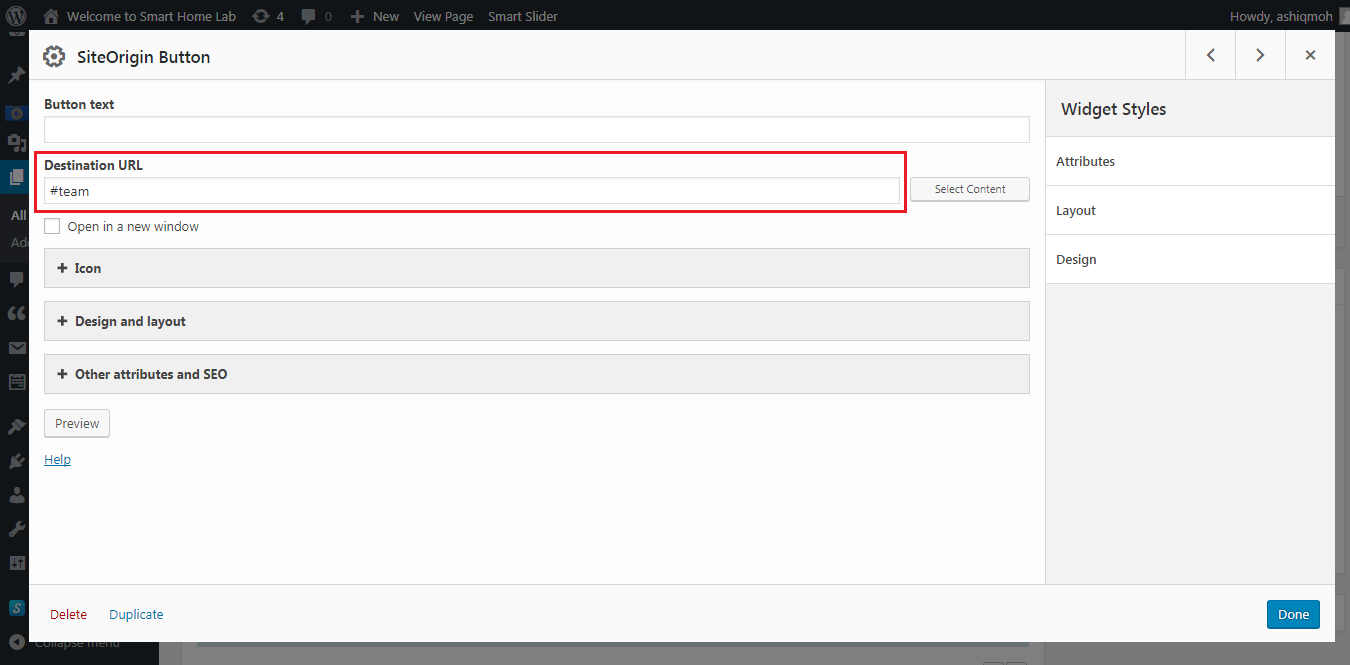
\includegraphics[height=5cm,keepaspectratio]{website-designing/destination-url-button.png}
\end{figure}

\begin{figure}[ht]
\caption{Adding Row Id to the Target Element}
\label{target-element-id}
\centering
	\begin{subfigure}{.49\linewidth}
	\centering
	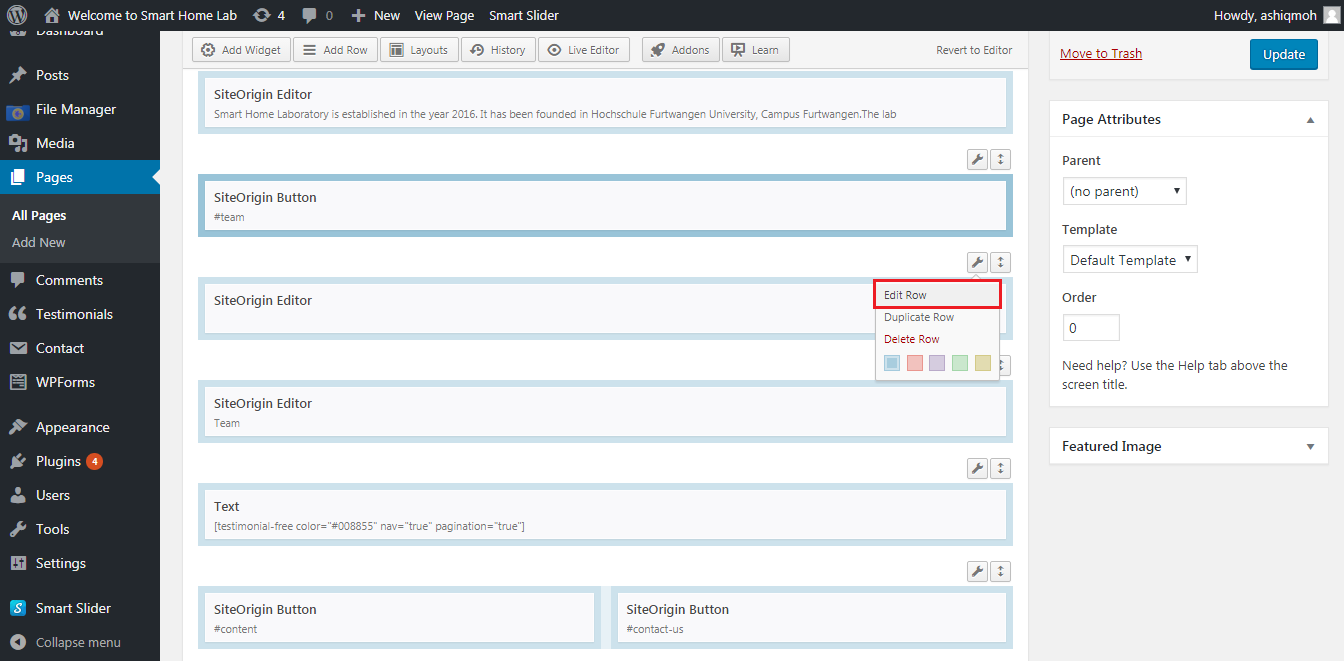
\includegraphics[width=\textwidth,keepaspectratio]{website-designing/destination-url-1.png}
	\end{subfigure}
	\begin{subfigure}{0.49\linewidth}
	\centering
	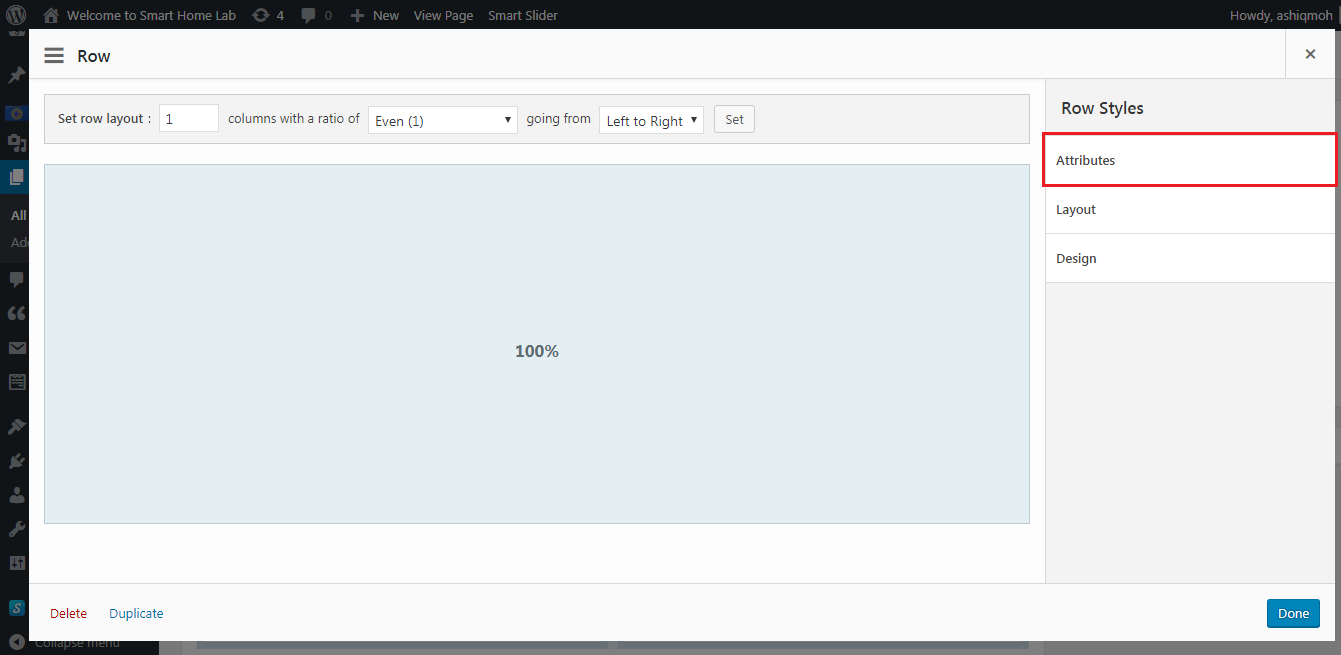
\includegraphics[width=\textwidth,,keepaspectratio]{website-designing/destination-url-2.png}
	\end{subfigure}
	\begin{subfigure}{0.49\linewidth}
	\centering
	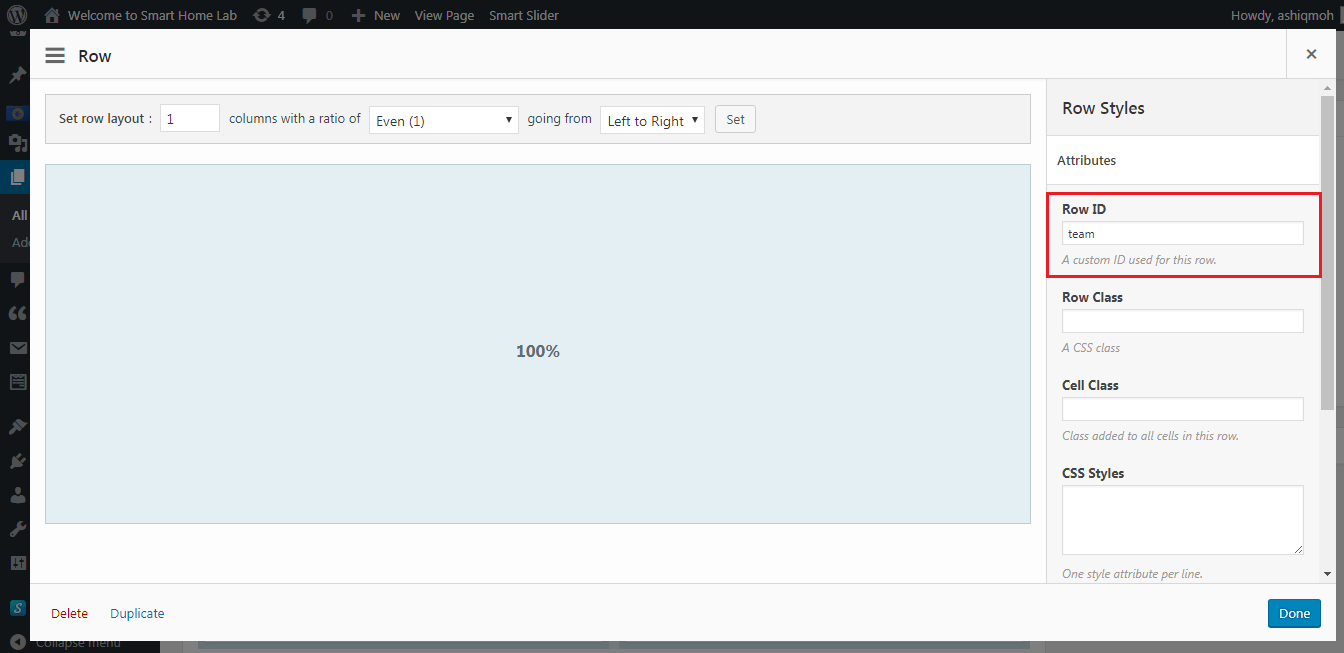
\includegraphics[width=\textwidth,,keepaspectratio]{website-designing/destination-url-3.png}
	\end{subfigure}
\end{figure}

\section{Adding ScrollReveal Effect}
ScrollReveal effect is an effect that can be added to the content of a web page, where the content will get an animation or effect that it is being revealed to the users as they scroll down or up through the page. This effect can be added to any website through importing a JavaScript library, ScrollReveal written by Julian Lloyd\footnote{https://scrollrevealjs.org/}.

This section will explain how to add this effect to a WordPress page. First, a plugin called 'Scripts n Styles'\footnote{https://wordpress.org/plugins/scripts-n-styles/} has to be added and activated in the WordPress. After activating the plugin, the 'Page' section in the WordPress will receive a new screen option under the editor, where JavaScript and CSS code can be added as shown in the Figure~\ref{scripts-n-styles}.

\begin{figure}[ht]
\centering
\caption{Scripts n Styles screen option}
\label{scripts-n-styles}
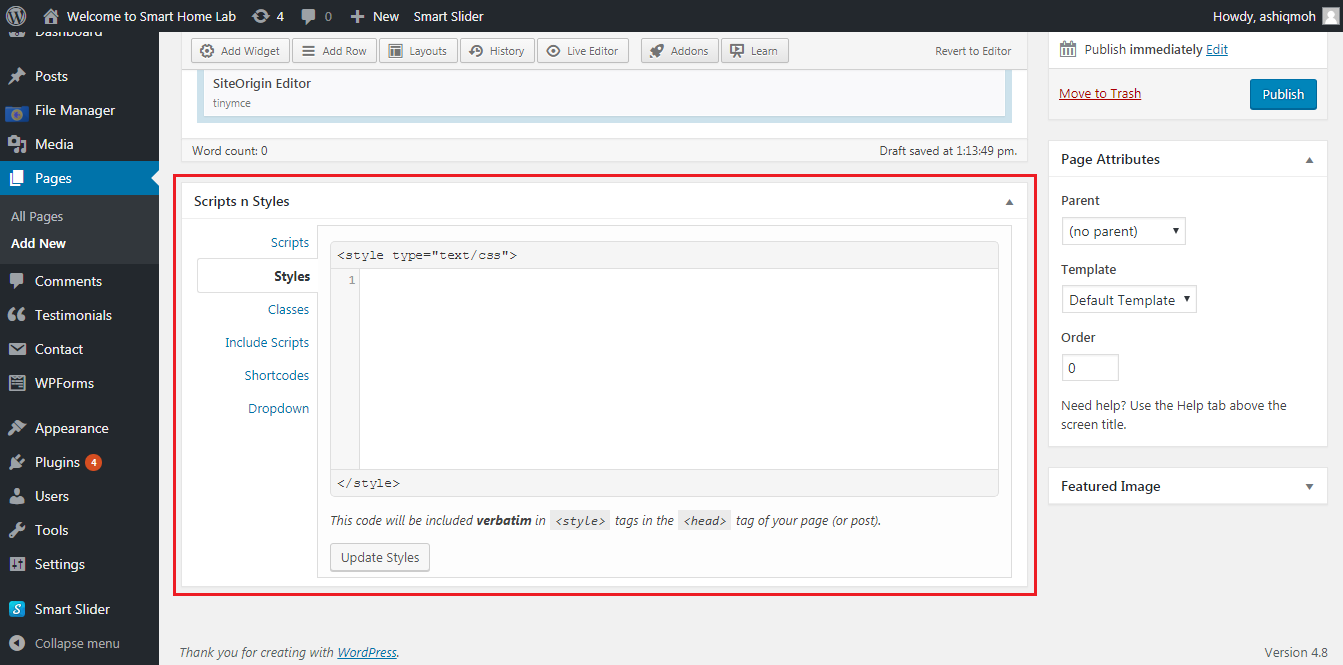
\includegraphics[height=5cm,keepaspectratio]{website-designing/scripts-n-styles.png}
\end{figure}

Here, the script tab has to be clicked so that our own JavaScript can be added to the current page. There, the plugin offers two option of adding JavaScript codes to current web page. Either at the header part of web page at the top, or at body part of the web page at the bottom. Here, the codes required to enable ScrollReveal effect will be added at the body of the web page at the bottom.

\begin{figure}[ht]
\centering
\caption{Adding JavaScript to bottom of page}
\label{javascript-bottom-column}
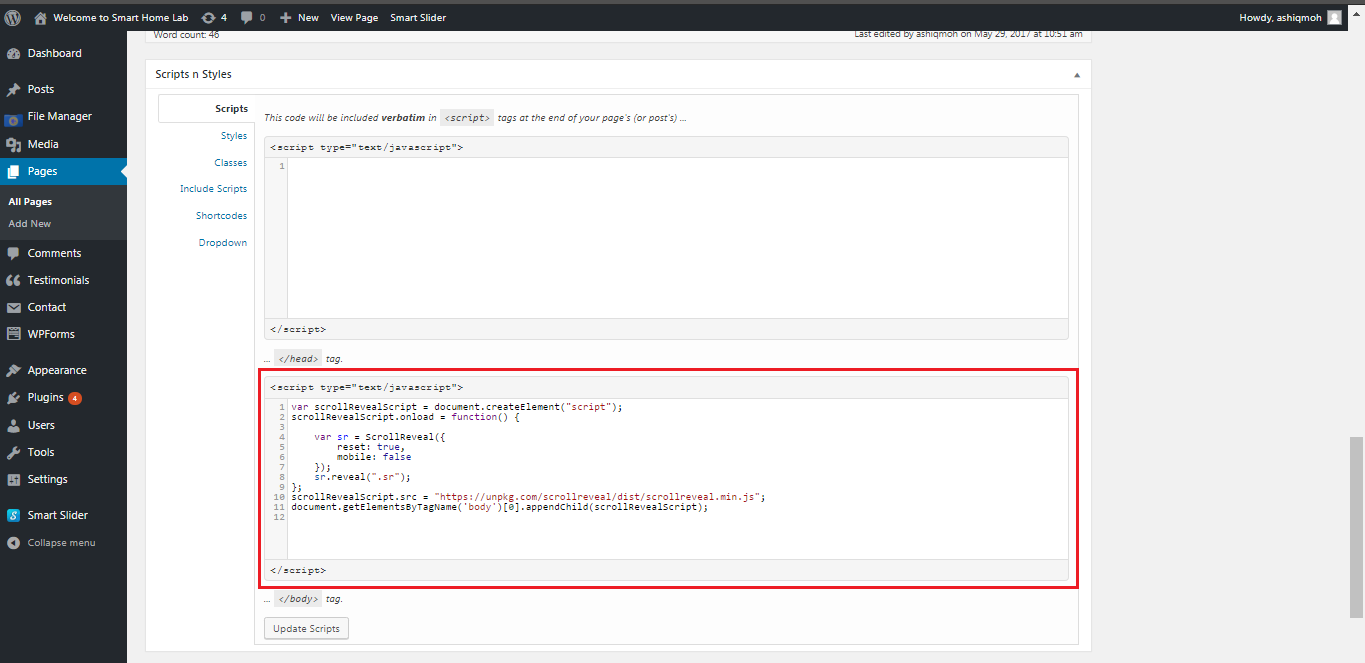
\includegraphics[height=5cm,keepaspectratio]{website-designing/javascript-bottom-column.png}
\end{figure}

The JavaScript codes that has been added will do two tasks. First, it will import the ScrollReveal library script from \ac{cdn} and insert it to current web page.

Secondly, the JavaScript code will be written to declare and initiate the ScrollReveal object, so that any HTML element assigned will receive the effect. Here, the elements with class name 'sr' has been assigned to get the ScrollReveal effect. The class name in JavaScript is identified with the punctuation mark '.' in the beginning. This has been done using the method \texttt{.reveal('.sr');}.

\begin{lstlisting}
var scrollRevealScript = document.createElement("script");
scrollRevealScript.onload = function() {

    // declare and initiate ScrollReveal object
    var sr = ScrollReveal({
        reset: true,
        mobile: false
    });
    // assign element that should receive the effect
    sr.reveal(".sr");
};
// import ScrollReveal library from CDN
scrollRevealScript.src = "https://unpkg.com/scrollreveal/dist/scrollreveal.min.js";
// insert the imported library into the web page
document.getElementsByTagName('body')[0].appendChild(scrollRevealScript);
\end{lstlisting}

The final step that has to be taken in order to enable the effect is to add the class name, in this case 'sr' to the HTML elements. This class name will be entered in the 'Row Class' field as shown in the Figure~\ref{class-name-sr}.

\begin{figure}[ht]
\caption{Adding Class Name to HTML Element}
\label{class-name-sr}
\centering
	\begin{subfigure}{.49\linewidth}
	\centering
	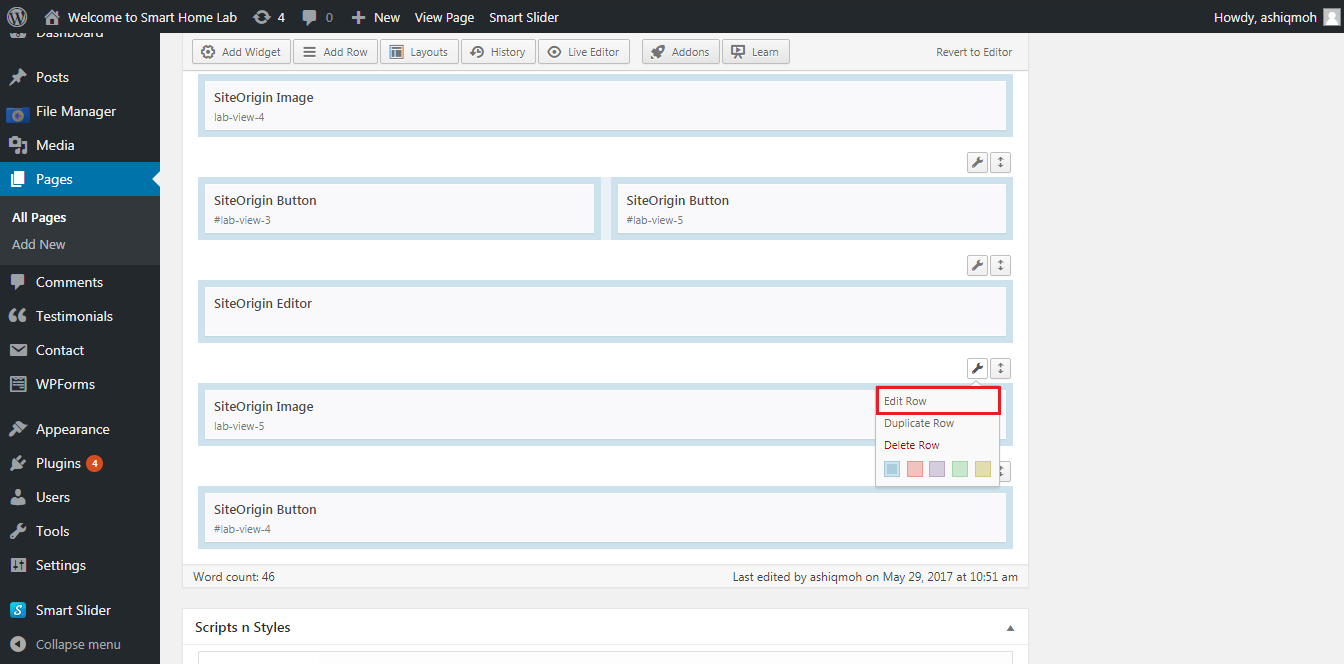
\includegraphics[width=\textwidth,keepaspectratio]{website-designing/class-name-sr-1.png}
	\end{subfigure}
	\begin{subfigure}{0.49\linewidth}
	\centering
	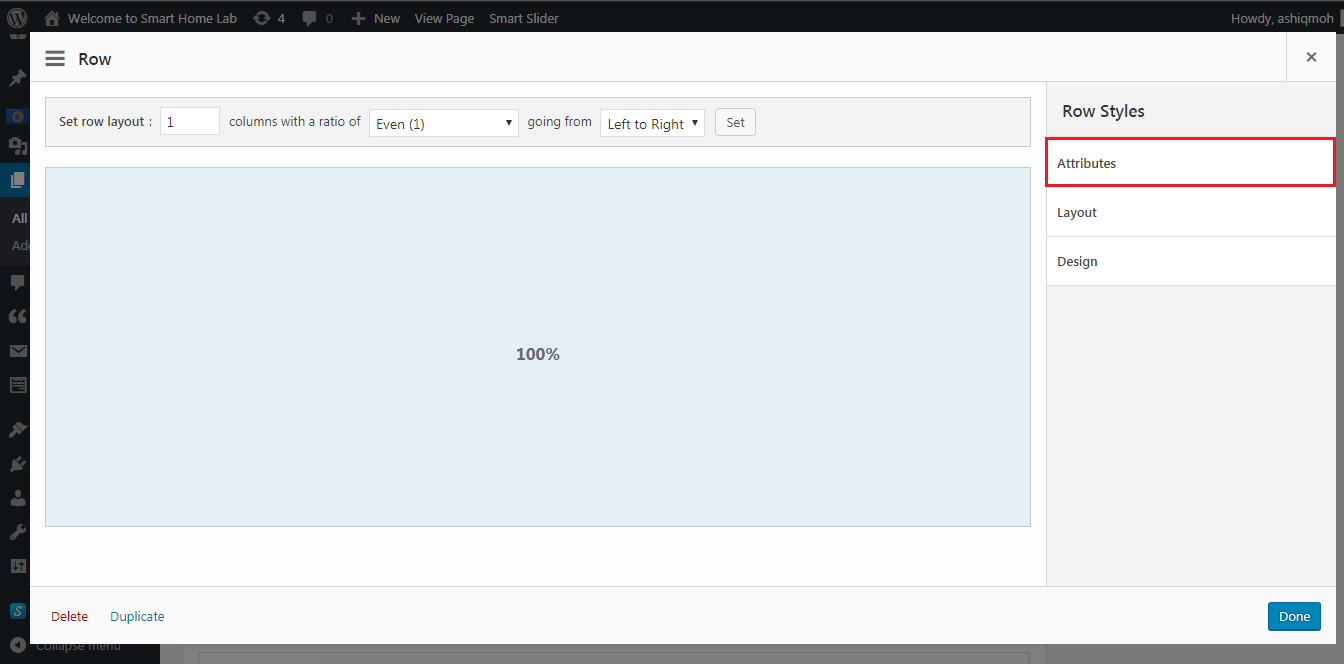
\includegraphics[width=\textwidth,,keepaspectratio]{website-designing/class-name-sr-2.png}
	\end{subfigure}
	\begin{subfigure}{0.49\linewidth}
	\centering
	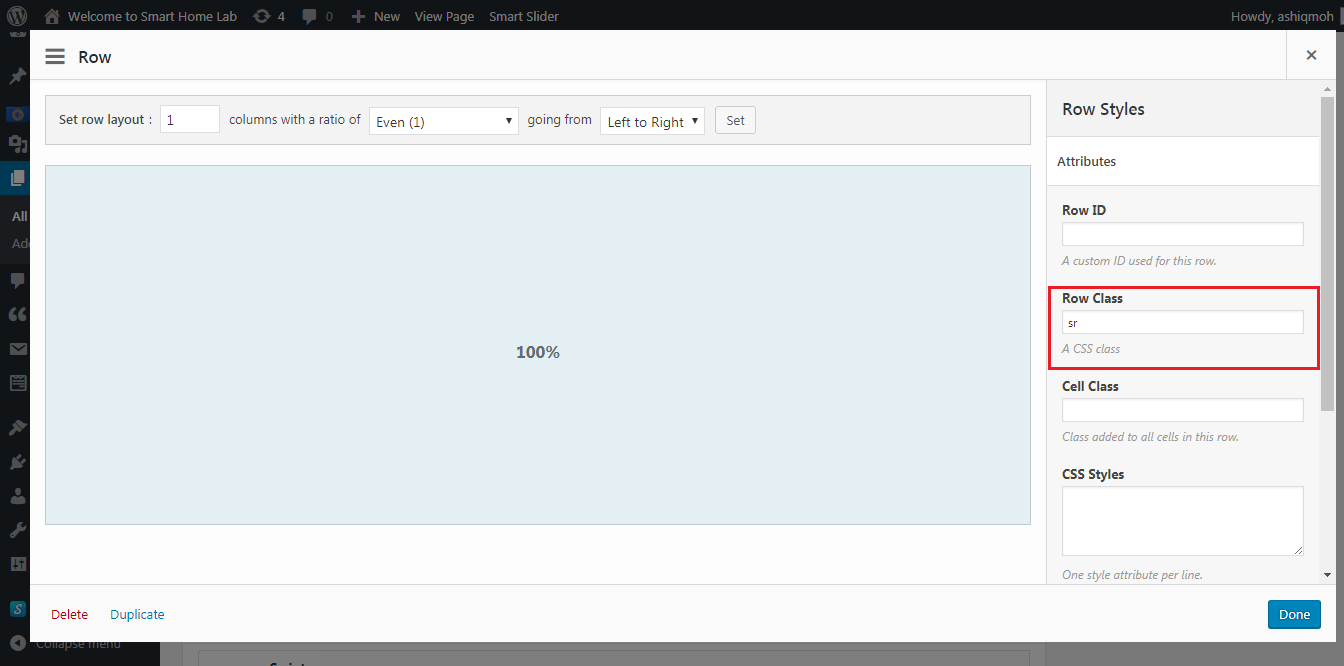
\includegraphics[width=\textwidth,,keepaspectratio]{website-designing/class-name-sr-3.png}
	\end{subfigure}
\end{figure}


\chapter{Implementation of the Info-Terminal}
The info-terminal has been created by using a \ac{wp} plugin called SmartSlider3\footnote{https://wordpress.org/plugins/smart-slider-3/}. SmartSlider3 is a free plugin available in the WordPress plugin repository. It enables the creation and designation of slider \cite{RefsnesData.8102017} easily with a lot of features.

\section{Getting Started}
First, the SmartSlider3 plugin has to be added and activated in the WordPress. After the activation, the left menu list will receive a new entry 'Smart Slider'. Click it will bring the Smart Slider dashboard interface, where slider can created, modified and deleted. A new slider can be created by clicking the 'New Slider' tile on the dashboard. Here the following details have been given:
\begin{itemize*}
\item Slide name: Info Terminal
\item Width: 1920 px
\item Height: 1080 px
\item Preset: Default
\item Import Sample Sliders: none
\end{itemize*}
\begin{figure}[ht]
\caption{Creating a new slider}
\label{creating-a-new-slider}
\centering
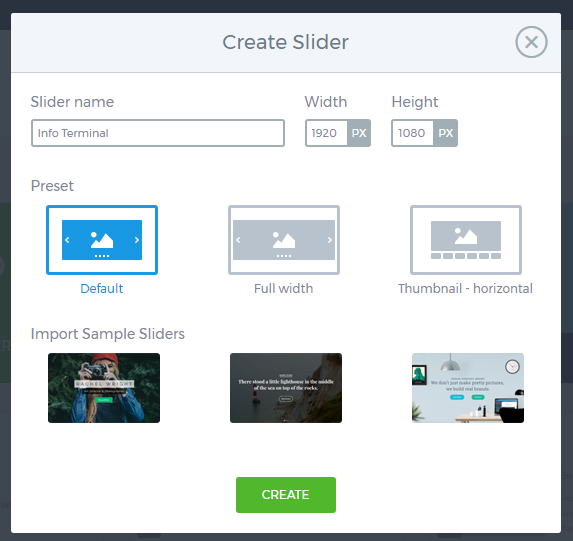
\includegraphics[height=4cm,keepaspectratio]{info-terminal/creating-new-slider.png}
\end{figure}

After the above mentioned details have been given, the creation of new slider have been proceed by clicking the 'Create' button.

\section{Slider Settings}
There are a few general settings that has to be configured after creating a new slider. The slider settings options can be found immediately after getting into the 'Info Terminal' slider.

subsection*{General Settings}
Under 'General' tab, two settings has be changed, which are:
\begin{itemize*}
\item Align: Center
\item Main animation properties (Duration): 600 ms
\end{itemize*}

\subsection*{Size Settings}
Here, the following attributes has to be changed:
\begin{itemize*}
\item Slide size (Width): 1920 px
\item Slide size (Height): 968 px
\item Slider height (Min): 300 px
\item Slider height (Max): 968 px
\item Slider width (max): 1920 px
\end{itemize*}

\subsection*{Autoplay Settings}
Here, the following attributes has to be changed:
\begin{itemize*}
\item Autoplay (Enabled): True
\item Autoplay (Interval): 5000 ms
\end{itemize*}

\subsection*{Arrow Settings}
Here, the following attributes has to be set:
\begin{itemize*}
\item Previous (Color): 999999FF
\item Style: Static
\end{itemize*}

\subsection*{Autoplay Icon Settings}
By default, the autoplay mode in the slider is turned off. This mode has to be turned on as shown in Figure~\ref{autoplay-icon-on} and the rest the of settings are left to default settings.
\begin{figure}[ht]
\caption{Autoplay Icon Settings}
\label{autoplay-icon-on}
\centering

\includegraphics[height=3cm,keepaspectratio]{info-terminal/autoplay-icon-on.png}
\end{figure}

\subsection*{Thumbnails Setting}
After enabling the Thumbnails, which by default is turned off, the following attributes have to be set.
\begin{itemize*}
\item Thumbnail size (Width): 150 px
\item Thumbnail size (Height): 100 px
\item Position: Outer, bottom
\end{itemize*}

\subsection*{Publish Setting}
Under the 'Publish' tab, the shortcode of the created slider has to be taken note (refer Figure~\ref{slider-shortcode}). In this case, the short code is \texttt{\[smartslider3 slider=1\]}. This code will be used to insert the slider into the WordPress web page as discussed in the Section~\ref{inserting-slider-into-web-page}.

\section{Inserting Slider Into Web Page} \label{inserting-slider-into-web-page}
A new WordPress page has to be created through the  \scalerel*{
\includegraphics{info-terminal/add-new-page.png}}{B} option under the \scalerel*{
\includegraphics{info-terminal/pages-menu.png}}{B} menu.
\begin{enumerate}
\item The title of page has been given as 'Info Terminal' in the 'Title' field.
\item The permalink or slug has been set to \texttt{info/}.
\item The shortcode, which have been noted down from previous section has to be pasted or typed in the editor.
\item Lastly, the template of this web page has been changed from 'Default Template' to 'Blank Slate'.
\end{enumerate}

\section{Creating and Setting Slide}
After setting the slider setting, slide can be created and set. The slider can be created by clicking the 'NEW SLIDE' green icon tile as shown in the Figure~\ref{new-slide-tile-icon}. After clicking it, we will be prompted to select an image. Here, any dummy image has to be chosen for time being until the slide background is set in the next step.
\begin{figure}[ht]
\caption{New slide tile icon}
\label{new-slide-tile-icon}
\centering

\includegraphics[height=2cm,keepaspectratio]{info-terminal/new-slide-tile-icon.png}
\end{figure}

Next, after the slide has been created, the following Background and Settings has to be given as shown in the Figure~\ref{slide-general-settings}. Through the 'Background' tab as shown in the Figure~\ref{slide-background}, these attributes has to be set to the following:
\begin{itemize*}
\item Background: Color
\item Color: FAFAFAFF
\end{itemize*}
Where else, through the 'Settings' tab, the name of the current slide along with the respective thumbnail can be inserted.
\begin{figure}[ht]
\caption{Slide settings}
\label{slide-general-settings}
\centering
	\begin{subfigure}{.49\linewidth}
	\caption{Slide background}
	\label{slide-background}
	\centering
	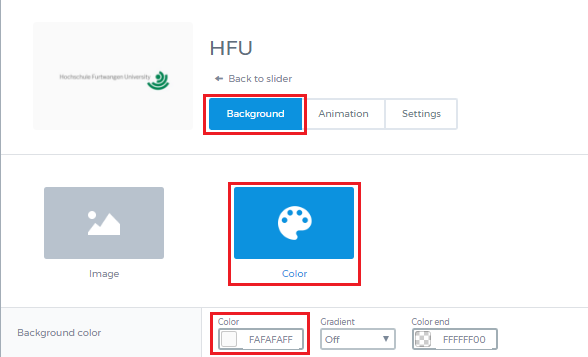
\includegraphics[height=3cm,keepaspectratio]{info-terminal/slide-background.png}
	\end{subfigure}
	\begin{subfigure}{.49\linewidth}
	\caption{Slide's name and thumbnail}
	\label{slide-settings}
	\centering
	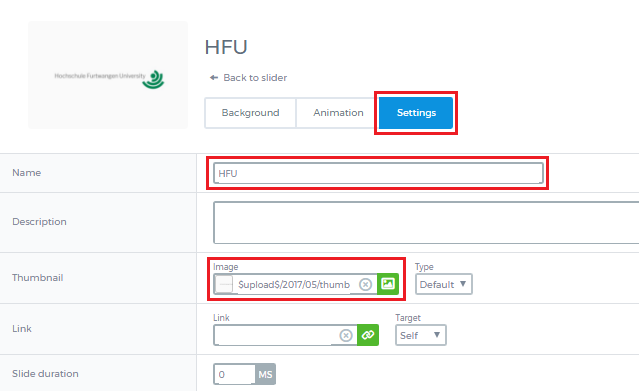
\includegraphics[height=3cm,keepaspectratio]{info-terminal/slide-settings.png}
	\end{subfigure}
\end{figure}

\section{Adding Home Button}
Home button has been added to all slides manually. The following steps explain how it is done in detail. First the 'Text layer' has to be added to the slide by clicking the \scalerel*{
\includegraphics{info-terminal/text-layer-icon.png}}{B} icon that can be found to the right of the slide view. This will bring up a widget (refer Figure~\ref{text-layer-widget}, where the following has to be set.
\begin{figure}[ht]
\caption{Text layer widget}
\label{text-layer-widget}
\centering
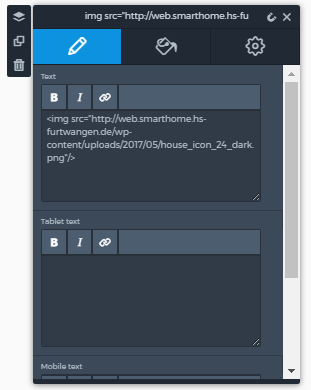
\includegraphics[height=3cm,keepaspectratio]{info-terminal/text-layer-widget.png}
\end{figure}

Through the first tab with icon \scalerel*{
\includegraphics{info-terminal/pencil-icon.png}}{B} in the 'Text' field, the following HTML codes has to be entered:
\begin{lstlisting}
<img src="http://web.smarthome.hs-furtwangen.de/wp-content/
      uploads/2017/05/house_icon_24_dark.png"/>
\end{lstlisting}

Through the third tab with icon \scalerel*{
\includegraphics{info-terminal/widget-gear-icon.png}}{B}, following has to be set:
\begin{itemize*}
\item Align: \scalerel*{
\includegraphics{info-terminal/home-button-align.png}}{B}
\item Position X: 25 px
\item Position Y: 25 px
\item Width: Auto
\item CSS class: home-button cursor-pointer
\end{itemize*}

Next, through the \scalerel*{
\includegraphics{info-terminal/pages-menu.png}}{B} menu, 'Edit' option has to clicked to open the 'Info Terminal' page, which has been created in the Section~\ref{inserting-slider-into-web-page}.

Under the 'Scripts n Styles' section, the following CSS codes has to be added under the 'Styles' tab:
\begin{lstlisting}
.cursor-pointer {
	cursor: pointer;
	text-decoration: none;
}
\end{lstlisting}

After that, under the 'Scripts' tab, the following \ac{js} codes has been added:
\begin{lstlisting}
window.n2ss.ready(1, function(slider){
	jQuery('.home-button').click(function(){
		window.location.href="/";
	});
});
\end{lstlisting}

These JavaScript codes give the callback functionality to the home button found on every slides. When, it is clicked, the browser takes the user to the website's home page.

\section{Adding Header} \label{sec:adding-header}
Header elements can be added into the slide by clicking on \scalerel*{
\includegraphics{info-terminal/header-icon.png}}{B} icon which can be found on the left side of the slide view. This will bring up a widget where the header text can be entered as shown in Figure~\ref{fig:info-terminal-adding-header-text}. By click the \scalerel*{
\includegraphics{info-terminal/widget-gear-icon.png}}{B} on the widget, the alignment, position and size (width, height) of the header element can be set, shown in Figure~\ref{fig:info-terminal-header-settings}.

\begin{figure}[ht]
	\begin{subfigure}{.49\textwidth}
	\caption{Adding header}
	\label{fig:info-terminal-adding-header-text}
	\centering
	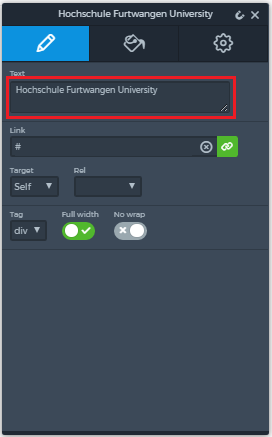
\includegraphics[height=3.5cm,keepaspectratio]{info-terminal/adding-header-element.png}
	\end{subfigure}
	\begin{subfigure}{.49\textwidth}
	\caption{Header element settings}
	\label{fig:info-terminal-header-settings}
	\centering
	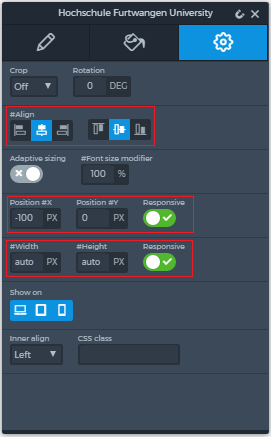
\includegraphics[height=3.5cm, keepaspectratio]{info-terminal/header-settings.png}
	\end{subfigure}
\end{figure}

\section{Adding Images}
Images can be added to slide by clicking the \scalerel*{
\includegraphics{info-terminal/image-icon.png}}{B} icon on left of the slide viewer. Clicking this icon will bring up the media selector window where an image has to be selected. After an image had been selected, the image widget can be seen with the selected image as shown in Figure~\ref{fig:image-widget}. Here also the gear icon can be selected to apply futher settings to the image such as positioning, alignment and sizing.

\begin{figure}[ht]
\caption{Image widget}
\label{fig:image-widget}
\centering
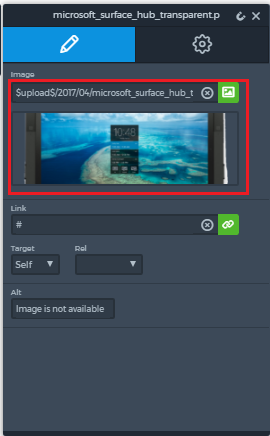
\includegraphics[height=3.5cm,keepaspectratio]{info-terminal/added-image.png}
\end{figure}

\section{Creating Overview Buttons}
Each spaces such as (living room, kitchen, washroom, workspace and multimedia room) will be presented with overview buttons as shown in Figure~\ref{fig:oveview-buttons}. This section will explain on how to create an overview button.

\begin{figure}[ht]
\caption{Overview buttons}
\label{fig:overview-button}
\centering
\includegraphics[height=3.5cm,keepaspectratio]{info-terminal/overview-buttons.png}
\end{figure}

\subsection*{Step 1: Adding Header Element}
An header element has to be added to slide as discussed in the Section~\ref{sec:adding-header}. Here the text should be given either 'Components', 'Panels' or 'Use Cases'. 

\subsection*{Step 2: Header Designing}
After adding a appropriate text, the header element has to be designed clicking the \scalerel*{\includegraphics{info-terminal/widget-paint-icon.png}}{B}. Clicking this, will show the CSS designing panel as shown in the Figure~\ref{fig:header-designing}. Here, the following design settings have to changed:
\begin{itemize*}
\item Color: FAFAFAFF
\item Line height: 5.75
\item Text align: \scalerel*{\includegraphics{info-terminal/align-center.png}}{B}
\item Background color: D85935FF (eg. for 'Components' button)
\item Border: 1 px Solid BB4A28FF (eg. for 'Components' button)
\item Border radius: 5 px
\end{itemize*}

\begin{figure}[ht]
\caption{Designing header element}
\label{fig:header-designing}
\centering
\includegraphics[height=3.5cm,keepaspectratio]{info-terminal/header-designing.png}
\end{figure}

subsection*{Step 3: Header Settings}
Next, the header element need to be set. The setting screen can be opened by clicking the \scalerel*{\includegraphics{info-terminal/widget-gear-icon.png}}{B}. Here besides alignment, positioning and sizing, the CSS class has to be set, which is important. In the CSS class text field as shown in Figure~\ref{fig:css-class-field}, the following text has to be entered:
\begin{lstlisting}
card-4 living-room-components
\end{lstlisting}

The \texttt{card-4} is constant for all overview button. The \texttt{living-room-} is depends on for which space the button are being added. For an example, for \emph{kitchen}, this part has to be replaced with \texttt{kitchen-}. The last part of is \texttt{components}. This part has to replaced accordingly. For an example, for \emph{panels}, this part should be replaced with \texttt{panels} and for \emph{use cases} with \texttt{use-cases}.

\begin{figure}[ht]
\caption{Adding CSS Class}
\label{fig:css-class-field}
\centering
\includegraphics[height=3.5cm,keepaspectratio]{info-terminal/css-class-field.png}
\end{figure}

Next by toggling to \emph{Hover} section by clicking \scalerel*{\includegraphics{info-terminal/design-hover.png}}{B} icon, the following entries have to be given:
\begin{itemize*}
\item Background color: BB4A28FF
\item Padding: 0 0 0 0 px
\item Border: 1 px Solid BB4A28FF
\item Border radius: 5 px
\end{itemize*}

\subsection*{Step 3: Adding CSS}
Next, click the \scalerel*{\includegraphics{info-terminal/pages-menu.png}}{B}. Then edit the 'Info-Terminal' page. Under the 'Style' tab in the 'Scripts n Styles' section, few lines of CSS codes have to be added for additional designing of the overview button as listed below:
\begin{lstlisting}
.card-4 {
	min-width: 19\%;
	min-height: 30\%;
	border-radius: 5px;
	box-shadow: 0 14px 28px rgba(0,0,0,0.25), 0 10px 10px rgba(0,0,0,0.22);
	cursor: pointer;
}

.card-4 div {
	position: absolute;
	min-width: 100\%;
	min-height: 100\%;
}
\end{lstlisting}

\subsection*{Step 4: Adding JavaScript Callback}
Lastly, a JavaScript callback has to be added to button, so that when the button is clicked, the slider takes the user to to respective slide. This can be done by adding the following code under the \emph{Script} tab under the \emph{Scripts n Styles} section.

\begin{lstlisting}
window.n2ss.ready(1, function(slider){
	jQuery('.living-room-components').click(function() {
		slider.slide(10);
	});
});
\end{lstlisting}

Above is an example of JavaScript callback implemented by using jQuery \texttt{.click} function. Here, the \texttt{'.living-room-components'} is the text entered in the CSS Class text field as discussed in the Step 3. The line \texttt{slider.slide(10)} is the execution telling the slider to move to slide number 10. Here, the destination slide is at index 10 starting with the first slide at index 0.

\section{Creating Component Buttons}
This section will discuss how to create the component buttons as shown in the Figure~\ref{fig:component-buttons}. The component buttons shown in figure belongs to the one that can be found in the living room. In this case, there are only two components in the living room, namely \emph{Surface Hub} and \emph{BenQ Smart Projector}. In order to create this buttons, there are few steps to be taken which will be discussed here.

\subsection*{Step 1: Adding header element}
Header element can be added to the slider by clicking the \scalerel*{\includegraphics{info-terminal/header-icon.png}}{B}. Then, the corresponding text has to be added to the \emph{Text} field which can be found on the widget first tab.

\subsection*{Step 2: Designing the header element}
Next, the header element has to be designed. To proceed with designing, click on the \scalerel*{\includegraphics{info-terminal/widget-paint-icon.png}}{B}. In this section of the widget as shown in the Figure~\ref{fig:component-button-designing}, following entries have to be changed:
\begin{itemize*}
\item Color: 414141FF
\item Line height: 1.5
\item Background color: CED3D5FF
\item Padding: 5 0 5 0 px
\item Border: 1 px solid 81898DFF
\item Border radius: 5px
\end{itemize*}

Next by toggling to \emph{Hover} section by clicking \scalerel*{\includegraphics{info-terminal/design-hover.png}}{B} icon, the following entries have to be given:
\begin{itemize*}
\item Background color: BDC1C3FF
\item Padding: 5 0 5 0 px
\item Border: 1 px Solid 81898DFF
\item Border radius: 5 px
\end{itemize*}

\begin{figure}[ht]
\caption{Designing component buttons}
\label{fig:component-button-designing}
\centering
\includegraphics[height=3.5cm,keepaspectratio]{info-terminal/component-button-designing.png}
\end{figure}

\subsection*{Step 3: Setting Header Element}
The header element has to be set with following settings. The setting panel of the header element can be opened by clicking the \scalerel*{\includegraphics{info-terminal/widget-gear-icon.png}}{B}. Here, the following entries has to be set:
\begin{itemize*}
\item Align:
\item Width: 1000 px
\item Height: auto
\item CSS claa: card-1 components-surface-hub
\end{itemize*}

CSS Class with text \texttt{card-1 components-surface-hub} is very important. The \texttt{card-1} is the reference to CSS styling which will be discussed in the next section. Whereby \texttt{components-surface-hub} is the reference for the JavaScript callback function. In this case, it refers to the destination slide which contains the component Surface Hub.

\subsection*{Adding CSS Styling}
To add the CSS styling for the component buttons, navigate to \scalerel*{\includegraphics{info-terminal/pages-menu.png}}{B}. Edit the \emph{Info Terminal}. Under the \emph{Styles} tab under \emph{Scripts n Styles} section, the following CSS codes have to be added:

\begin{lstlisting}
.card-1 {
	border-radius: 5px;
	box-shadow: 0 5px 10px rgba(0,0,0,0.19), 0 6px 6px rgba(0,0,0,0.23);
	cursor: pointer;
}
\end{lstlisting}

\subsection*{Adding JavaScript Callback}
The JavaScript callback is a small codes that will get executed when the user click on the component buttons. This codes will be added to the \emph{Scripts} tab under the \emph{Scripts n Styles} section. Here, the following codes have to be added:

\begin{lstlisting}
window.n2ss.ready(1, function(slider){
	jQuery('.components-surface-hub').click(function(){
		slider.slide(11);
	});
});
\end{lstlisting}

The example callback function above contains the reference \path{'.components-surface-hub'}. When the button with this reference get clicked, the \texttt{.click()} function will be executed which will slide the slider to to slide with index 10. The slide number 10 should contain, in this case, the \emph{Surface Hub}. The index counting starts from 0.

\section{Creating Panel Buttons}
This section will explain on how to create a panel button as shown in the Figure~\ref{fig:panel-buttons}. Panel buttons are buttons that have been used as navigation to items that can be found on the panels in the lab. These buttons have been created with images of item itself.

\begin{figure}[ht]
\caption{Panel buttons}
\label{fig:panel-buttons}
\centering
\includegraphics[height=3.5cm,keepaspectratio]{info-terminal/panel-buttons.png}
\end{figure}

\subsection*{Step 1: Adding Text Layer}
In order to add or create a panel button, a text layer has to be added by clicking \scalerel*{\includegraphics{info-terminal/text-layer-icon.png}}{B} icon that can be found on left of the slide viewer. This is bring up the text layer widget as shown in the Figure~\ref{fig:text-layer-widget}. In the \emph{Text} field which can be found under \scalerel*{\includegraphics{info-terminal/pencil-icon.png}}{B}, the following HTML codes have to be added. This code will result in the following button containing the Sonos Play:5 speaker as the button image.

\begin{lstlisting}
<div class="panel-nav-container panels-sonos-play5">
	<span class="span-helper"></span>
	<img src="/wp-content/uploads/2017/04/play5-blk-angle.png" alt="Sonos Play:5" style="vertical-align:middle;max-width:75%;max-height:75%;">
</div>
\end{lstlisting}

\subsection*{Step 2: Setting of Text Layer}
Setting of the text layer can be accessed by clicking the \scalerel*{\includegraphics{info-terminal/widget-gear-icon.png}}{B}. Here, only two settings has to be changed as listed below:
\begin{itemize*}
\item Width: 200 px
\item Height: 200 px
\end{itemize*}

Apart from the width and height, the positioning of the button in X and Y direction has to be set accordingly as can be seen in Figure~\ref{fig:panel-buttons}.

\subsection*{Step 3: Adding CSS Styling}
To style the button, CSS styling has to applied. Edit the \emph{Info Terminal} page which can be found under \scalerel*{\includegraphics{info-terminal/pages-menu.png}}{B}. Under the \emph{Styles} tab under \emph{Scripts n Styles} section, the following CSS code has to be added:
\begin{lstlisting}
.panel-nav-container {
	background-color: #fff;
	text-align: center;
	width: 100%;
	height: 100%;
	border-radius: 10px;
	border: 1px solid #aaa;
	box-shadow: 0 0 5px 2px rgba(0, 0, 0, 0.2) inset;
	cursor: pointer;
	position: absolute;
}

.panel-nav-container:hover {
	border: 1px solid #008855;
	box-shadow: 0 0 5px 2px rgba(0, 136, 85, 0.2) inset;
}

.span-helper {
	display: inline-block;
	height: 100%;
	vertical-align: middle;
}

.panel-nav-container img {
	transform: scale(1);
	transition: transform 0.5s;
	transition-timing-function: ease;
}

.panel-nav-container:hover img {
	transform: scale(1.1);
}
\end{lstlisting}

This CSS code will style the panel button and the image of button as well. The CSS with \emph{:hover} tags add the hover effect to buttons.

\subsection*{Step 4: Adding JavaScript Callback}
Lastly, the JavaScript callback function has to be added to the button when the user click on the buttons. The JavaScript callback has to be added under the \emph{Scripts} tab under the \emph{Scripts n Styles} section of the \emph{Info Terminal} page.
\begin{lstlisting}
window.n2ss.ready(1, function(slider){
	jQuery('.panels-sonos-play5-2').click(function(){
		slider.slide(55);
	});
});
\end{lstlisting}

\section{Creating Use-Cases Buttons}
Use-cases buttons are the buttons used to navigate user to the use-cases that can be found in the lab. A use-case button contains an image and a short descriptive text below the text as shown in Figure~\ref{fig:use-cases-buttons}

\begin{figure}[ht]
\caption{Use-cases buttons}
\label{fig:use-cases-buttons}
\centering
\includegraphics[height=3.5cm,keepaspectratio]{info-terminal/use-cases-buttons.png}
\end{figure}

\subsection*{Step 1: Adding Text Layer}
Begin by adding the text layer to the slide by clicking the \scalerel*{\includegraphics{info-terminal/text-layer-icon.png}}{B}. In the \emph{Text} field under the \scalerel*{\includegraphics{info-terminal/pencil-icon.png}}{B} the following HTML codes have to be entered:

\begin{lstlisting}
<img src="/wp-content/uploads/2017/05/window-light-on.jpg" alt="Window Lighting" style="width:400px;">
<div class="use-cases-desc">
	<p>Window Ligthing</p>
</div>
\end{lstlisting}

The above code is an example of use-cases button for \emph{Window Lighting}.

\subsection*{Step 2: Adding CSS Class}
After adding the HTML codes to the \emph{Text} field, class text has to be added to the \emph{CSS class} field which can be found under the  \scalerel*{\includegraphics{info-terminal/widget-gear-icon.png}}{B}. Here the following CSS class has to be entered:
\begin{lstlisting}
use-cases-container use-cases-window-ligthing
\end{lstlisting}

The \texttt{use-cases-container} will be used as a reference for CSS styling. And the \texttt{use-cases-window-lighting}, in this case as an example for window lighting use-cases button, will be used as CSS class reference for the JavaScript callback.

\subsection*{Step 3: Adding CSS Styling}
The use-cases buttons have been styled by using custom CSS code. The CSS code has been entered under the \emph{Styles} tab under the \emph{Scripts n Styles} section of the \emph{Info Terminal} page. The following CSS code has been added for styling:
\begin{lstlisting}
div.use-cases-container {
	max-width: 20%;
	background-color: white;
	box-shadow: 0 4px 8px 0 rgba(0, 0, 0, 0.2);
	cursor: pointer;
	transition: box-shadow 0.5s;
	transition-timing-function: ease;
}

div.use-cases-desc {
	border-top: 1px solid #aaa;
	text-align: center;
	padding: 3.5% 5.5%;
}

div.use-cases-container:hover {
	box-shadow: 0 10px 20px 5px rgba(0, 0, 0, 0.2);
}
\end{lstlisting}

\subsection*{Step 4: Adding JavaScript Callback}
Lastly, JavaScript callback has to be programmed so that the slider will navigate to the destination slide when the user click on the use-cases buttons. The JavaScript callback script has to be added under the \emph{Scripts} tab under the \emph{Scripts n Styles}.

\begin{lstlisting}
window.n2ss.ready(1, function(slider){
	jQuery('.use-cases-window-ligthing').click(function(){
		slider.slide(62);
	});
	jQuery('.use-cases-rainbow-ligthing').click(function(){
		slider.slide(63);
	});
});
\end{lstlisting}

\section{Creating Breadcrumb}
Breadcrumb, as shown in the Figure~\ref{fig:breadcrumb}, is the navigation bar that can be found on the slides, where user can navigate from the current level to the upper hierarchy level.

\begin{figure}[ht]
\caption{Breadcrumb}
\label{fig:breadcrumb}
\centering
\includegraphics[height=2.5cm,keepaspectratio]{info-terminal/breadcrumb.png}
\end{figure}

\subsection*{Step 1: Adding Text Layer}
Start creating a breadcrumb by adding a text layer to the slide by clicking \scalerel*{\includegraphics{info-terminal/text-layer-icon.png}}{B} icon

\begin{lstlisting}
<span class="breadcrumb_link breadcrumb-lab">Lab</span> / <span class="breadcrumb_link lab-multimedia-room">Multimedia Room</span> / Use Cases
\end{lstlisting}

\subsection*{Step 2: Adding CSS Styling}
Next, CSS styling has to be applied. The CSS code has to entered unde the \emph{Styles} tab under the \emph{Scripts n Styles} section in the Info Terminal page.

\begin{lstlisting}
.breadcrumb_link {
	color: #337ab7;
	cursor: pointer;
}

.breadcrumb_link:hover {
	filter: brightness(70%);
	text-decoration: underline;
}
\end{lstlisting}

\subsection*{Step 3: Adding JavaScript Callback}
Lastly, JavaScript callback script has to be added so that when the user click on the breadcrumb link, the slider will take user to the destination slide.
\begin{lstlisting}
window.n2ss.ready(1, function(slider){
	jQuery('.breadcrumb-lab').click(function(){
		slider.slide(4);
	});
});
\end{lstlisting}
\chapter{CCTV Live Stream}

\section{Introduction}
Another task in this thesis work is to stream live \ac{cctv} footage on the website. The CCTV used in thesis work is called PremiumBlue IP Camera \cite{PremiumBlue.2013} \cite{PremiumBlue.2013b} as shown in the Figure~\ref{fig:premium-blue-ip-camera}. This camera is built with 720p resolutions, can be rotated and tilted remotely and monitored wirelessly. It is suitable to be used in homes, offices and labs. The user interface of the camera, which is used to view the footage and control the camera itself, can be accessed through the web browser. Additionally, it has a SD-card slot, which enables the storing of the footages and replay of them in the later time.

\begin{figure}[ht]
\caption{PremiumBlue IP-Camera}
\label{fig:premium-blue-ip-camera}
\centering
\includegraphics[height=3.5cm,keepaspectratio]{cctv/premium-blue-ip-camera.jpg}
\end{figure}

This chapter will discuss on how to configure the above mentioned IP-Camera; extracting the information to get the camera footage and controlling the camera; and designing the web page in the WordPress.

\section{Pre-Configuration}
\subsection{Identifying IP Address}\label{sec:cctv-identifying-ip-address}
\emph{The steps discussed here is part of configuration steps from the camera vendor, which can be found in the following documentation}\cite{PremiumBlue.2013c}.\\

The camera came with built-in web application and a bundle of softwares. To get started, the IP-Camera need to be connected to power supply and LAN-network. Next, we need to identify the \ac{ip} of the camera by using the software came bundled with the camera called \emph{SearchIPCam.exe} (\emph{see} Figure \ref{search-ip-cam-exe}). This application can also be downloaded from the vendor's website\footnote{https://www.pollin.de/shop/downloads/D722622S.ZIP}. Run the program and hit the 'Refresh' button to obtain the IP address of the camera.

\begin{figure}[ht]
\caption{SearchIPCam.exe}
\label{search-ip-cam-exe}
\centering
	\begin{subfigure}{.49\linewidth}
	\includegraphics[width=\textwidth]{cctv/search-ip-cam-cropped.png}
	\end{subfigure}
	\begin{subfigure}{.49\textwidth}
	\includegraphics[width=\textwidth]{cctv/search-ip.png}
	\end{subfigure}
\end{figure}

\subsection{Login into Web Interface}
After identifying the IP address of the camera, the web interface of the camera can be accessed by giving in the identified IP address (e.g. 192.168.0.157) from previous step in the web browser's address bar. Login by using the following credentials.
\begin{itemize*}
\item Anwender: admin
\item Passwort: admin
\item Modus: Server Push
\end{itemize*}
(Note: 'Anwender' and 'Passwort' were not changed as at time of writing this. It may be changed in the future.)

\begin{figure}[ht]
\caption{Login in into IP-Camera web interface}
\label{ip-camera-web-interface}
\centering
\includegraphics[width=.7\linewidth,keepaspectratio]{cctv/web-interface-login.png}
\end{figure}

\subsection{WLAN Setup}
After successful login, the settings of the IP Camera can be accessed by clicking the tool button 'Einstellung' on top right of the page. In the menu list on the left panel, click on the 'WLan'. In there search for the available WLAN network by clicking the 'Suchen' button. After the program finish the search, choose the lab network identified by \ac{ssid} name 'SHLAB01' or 'SHLAB02'. Enter the following details:
\begin{itemize*}
\item WLan wird verwendet: tick
\item SSID: 'SHLAB01' or 'SHLAB02'
\item Netzwerk Type: Infra
\item Sicherer Modus: AEP
\item Verschl\"usselung: WPA2-PSK
\item Key: 91054319
\end{itemize*}
Hit the 'Update' and 'Speichern' buttons and close the web browser or the tab. (Note: The SSID and password may be changed in the future time.)
\begin{figure}[ht]
\caption{IP-Camera WLAN settings}
\label{ip-camera-wlan-settings}
\centering
	\begin{subfigure}{.34\textwidth}
	\includegraphics[width=\textwidth]{cctv/ip-camera-setting-button.png}
	\end{subfigure}
	\begin{subfigure}{.63\textwidth}
	\includegraphics[width=\textwidth]{cctv/wlan-search.png}
	\end{subfigure}
\end{figure}
\begin{figure}[ht]
\caption{WLan Credentials}
\label{wlan-credentials}
\centering
\includegraphics[width=.6\textwidth]{cctv/wlan-credentials.png}
\end{figure}

\subsection{Restart}
Now, the IP-Camera has to be restarted without connecting it to network via \ac{lan} cable. Since the wireless network credentials have been entered in the previous step, it will connect to lab network, 'SHLAB02' automatically upon start-up and will have a different IP address. Run the \emph{SearchIPCam.exe} program again as discussed in the Section~\ref{sec:cctv-identifying-ip-address} and login into the web interface using the new IP address. The IP address will be renewed when the IP-Camera is connected through wireless LAN.

\section{Identifying the cgi-bin Module}
\subsection{Introduction}
In order to stream the live footage or recording of the IP-Camera in the Smart Home Lab website, the URI address and additional query parameters are required in order to access the IP-Camera recording. These parameters are not available openly but can be obtained by studying the HTML and JavaScript codes of the web interface of the camera. The studying of the web interface codes may take time up to 1 to 2 days depending on the level of web programming knowledge. The URI where the footage of the camera can be obtained is identified with relative path \emph{cgi-bin}.

\subsection{Studying the Codes}\label{sec:cctv-studying-the-codes}
The codes can be studied by using the \emph{Developer Mode} of any web browser. In this thesis, the Chrome web browser has been used. The developer mode of Chrome web browser can be opened either through (Right click {\textgreater} Inspect) option or keyboard shortcut key (Ctrl-Shift-I).

The the HTML and JavaScript codes of the IP-Camera web interface, however, can't be studied easily because the are a lot of files which are embedded upon one another and referred to and from one file to another. The method used to extract the required \ac{uri} and query parameters are through backtracking the video footage and the callback functions of the controller buttons.

Upon successful backtracking, the video footage can be found out to be delivered through the following URI:
\newline
\texttt{\footnotesize{http://\textless base\_uri\textgreater/cgi-bin/videostream.cgi?user=\textless username\textgreater\&pwd=\textless password\textgreater}}
\newline
Where,
\begin{itemize*}
\item base\_url: 192.168.0.157 (\emph{as per SearchIPCam.exe search result})
\item username: admin
\item password: admin
\end{itemize*}

\begin{figure}[ht]
\caption{Developer Mode panel Sources}
\label{developer-mode-panel-sources}
\centering
\includegraphics[width=\linewidth,keepaspectratio]{cctv/controller-backtrack.png}
\end{figure}

The \ac{uri} required to control the camera (panning and tilting), can be backtracked through the controller buttons. The backtrack will lead to a function called \texttt{all\_ptz\_control(type, value)} in the \texttt{live.htm} file. This file can be found through the developer mode panel \emph{Sources}. Expand content\_frame (ffserver.htm) \textgreater push\_content\_frame (live.htm) \textgreater 192.168.0.157 nodes to find and open that file (see Figure \ref{developer-mode-panel-sources}).

After opening the file, the function can be found either through manual scrolling and searching or through search functionality that can be invoked through keyboard shortcut key (Ctrl-F). Through this function, the required URI to control the camera can be found out, which is:
\newline
\path{http://<base_uri>/cgi-bin/decoder_control.cgi?type=<type>&cmd=}
\newline
\path{<command>user=<username>&pwd=<password>}
\newline
Where,
\begin{itemize*}
\item base\_uri: 192.168.0.157 (\emph{as per SearchIPCam.exe search result})
\item type: 0
\item command: \emph{see Table \ref{camera-control-commands}}
\item username: admin
\item password: admin
\end{itemize*}

\begin{table}[ht]
\centering
\caption{Camera Control Commands}
\label{camera-control-commands}
\begin{tabular}{|l|l|}
\hline
Command & Camera Movement \\
\hline
0 & Up \\
1 & Down \\
2 & Right \\
3 & Left \\
10 & Stop \\
11 & Centralize \\
13 & Up-Left \\
14 & Down-Left \\
15 & Up-Right \\
16 & Down-Right\\
\hline
\end{tabular}
\end{table}

\section{Designing the Web Page}\label{sec:cctv-designing-the-web-page}
\subsection{Introduction}
In this section, the process of designing the web page to stream live footage of CCTV or IP-Camera will be discussed. In order to design this page, WordPress, CSS, JavaScript and jQuery knowledge will be required. In general, the development involves styling with CSS. Additionally, JavaScript will be used to render the HTML view, handle user actions and execute \ac{ajax} request.

\subsection{Creating the Web Page}
The web page is created by using WordPress built-in functionality. To create a new page, go to 'Page' section from the left side menu and click on 'Add New' sub-menu. Here, the page name is given as 'Live Stream' and then the page is published by clicking 'Publish' button. All the other settings are left in the default mode.

\subsection{Scripts n Styles Plugin}
Next, JavaScript \cite{Rauschmayer.2014} code will be added to render the HTML view. Below the WordPress text editor column, the 'Scripts n Styles' column can be found (\emph{refer} Figure~\ref{fig:scripts-n-styles-column}). This column will be added to every created page because of the installation of a WordPress plugin by the same name, 'Scripts n Styles'. To find out about the installed and activated plugins, explore the Plugins page. To learn more about this plugin, refer to URL linked in given footnote\footnote{https://de.wordpress.org/plugins/scripts-n-styles/}. Basically, this plugin enable the WordPress user to add custom CSS and JavaScript codes globally or to individual pages. Custom CSS and JavaScript is added into the page created to render the IP-Camera recording and the controller buttons.

\begin{figure}[ht]
\caption{Scripts n Styles Column}
\label{fig:scripts-n-styles-column}
\centering
\includegraphics[width=.7\linewidth,keepaspectratio]{cctv/scripts-n-styles-column.png}
\end{figure}

\subsection{Self-Invoked JavaScript Function}
First, a self-invoked JavaScript function will be added into 'Scripts' lower column as shown in the Figure~\ref{fig:scripts-n-styles-column}. The self-invoked JavaScript will be executed by the browser as soon as the script has been loaded without being called. This function contains codes to render the HTML view, which will render a HTML form with 3 input text fields:
\begin{itemize*}
\item IP
\item Username
\item Password
\end{itemize*}
and a submit button The rendered view will then be inserted into HTML page under the \texttt{div} element with class name \texttt{'entry-content'}.

\begin{figure}[ht]
\caption{HTML form with 3 input text fields and a submit button}
\label{fig:html-view-cctv-form}
\centering
\includegraphics[width=.7\linewidth,keepaspectratio]{cctv/html-view-cctv-form.png}
\end{figure}

In addition to that, the function has the callback method to handle when the form is submitted by the user. The codes can be found within the function block as shown below.
\begin{lstlisting}
// self-invoked function to run when page is loaded
(function () {
	// codes to render view and form submission
	...
	...
})();
\end{lstlisting}

\subsection{Rendering CCTV Footage and Controller} \label{sec:cctv-rendering-camera-module}
After the form as shown in Figure~\ref{fig:html-view-cctv-form} is submitted by user, the JavaScript will execute the codes to render the CCTV footage view and controller buttons. The rendering of these elements is handled by a function with the name \texttt{CameraModule}. This function is divided into 3 sub-functions:
\begin{itemize*}
\item \texttt{init()}
\item \texttt{renderStream()}
\item \texttt{renderController()}
\end{itemize*}

\begin{lstlisting}
const CameraModule = {};

CameraModule.init = function () {
	// codes
	...
}
CameraModule.renderStream = function () {
	// codes
	...
}
CameraModule.renderController = function () {
	// codes
	...
}
\end{lstlisting}

\begin{figure}[ht]
\caption{Camera Module HTML View}
\label{fig:camera-module-html-view}
\centering
\includegraphics[width=.6\linewidth,keepaspectratio]{cctv/camera-module-html-view.png}
\end{figure}

These sub-functions contain codes to execute what their name suggest. The \texttt{init()} has codes to initialize the HTML view rendering process by clearing the current view and setting the text fields input values from the HTML form in the functional scope variables. The \texttt{renderStream()} function render the camera footage stream, and the \texttt{renderController()} renders the controller buttons into the view. The rendered HTML view will appears as shown in the Figure~\ref{fig:camera-module-html-view}.

\subsection{Styling and Positioning the Buttons}
The controller buttons that are rendered through JavaScript alone do not appear as shown in Figure~\ref{fig:camera-module-html-view}. In order to make them appear good and positioned in a group as such, some CSS styling and positioning have been done. The CSS codes used for this purpose can be viewed from 'Styles' section of the 'Scripts n Styles' column.

The positioning of the buttons are done through relative and absolute positioning mechanism of the CSS\footnote{https://www.mediaevent.de/tutorial/css-position-absolute-relative.html}. In addition to that, the buttons has to be given the position as where it should find itself within the button container. The direction of arrow, as to which direction it should be pointing is done through CSS-Transform rotate effect.

\begin{lstlisting}
/* relatively positioned button container */
.btn-container {
	position: relative;
	width: 200px;
	height: 200px;
}

/* absolutely positioned buttons */
.navi-btn {
	line-height: 0;
	padding: 8px;
	position: absolute;
}

/* position of button in the button container */
.btn-top {
	top: 0;
	left: 72px;
}

... /* positioning of other buttons */

/* arrow direction of the button */
.arrow-down {
	-webkit-transform:rotate(180deg);
	-moz-transform: rotate(180deg);
	-ms-transform: rotate(180deg);
	-o-transform: rotate(180deg);
	transform: rotate(180deg);
}

... /* arrow positioning of other buttons */
\end{lstlisting}

\subsection{Callback Functions}
The last thing that needed to be added to this web page is the callback functions. Callback functions here refers to what should be done when the controller buttons are clicked using mouse or pressed using touch display such as on smartphone. The controller buttons remotely control the movement of the camera. All the buttons are registered with 4 types of event handlers except for the middle button, which has only 2 event handlers.

The 4 event handlers registered are as follow:
\begin{itemize*}
\item onmousedown - when user click the mouse left button
\item onmouseup - when user lift the clicking of mouse left button
\item ontouchstart - when user start the touch of button (touch display)
\item ontouchend - when user end the touch of button (touch display)
\end{itemize*}

The 2 event handlers registered for center button are as follow:
\begin{itemize*}
\item onclick - when user click on the button
\item ontouch - when user touch on the button
\end{itemize*}

All these event handlers are registered on the respective buttons during the rendering process as discussed in the Section~\ref{sec:cctv-rendering-camera-module}. The registering is done through the JavaScript method \texttt{setAttribute()}. This method register the event handler and the callback function to be invoked as shown in the code example below.

\begin{lstlisting}
// .setAttribute(event_handler, callback_fn);
btn.setAttribute('onmouseup', 'navi_stop(event)');
\end{lstlisting}

For these buttons, only 2 callback functions are required. First is the callback function when the events 'onmousedown', 'ontouchstart', 'onclick', and 'ontouch' are detected. Second callback function is when the event 'onmouseup' and 'ontouchend' are detected. The first callback function, \texttt{navi\_start(event, command} contain codes to make AJAX request to the IP-Camera for starting the navigation as per user command. The second callback function, \texttt{navi\_stop(event)} contain codes to make AJAX request to the IP-Camera to stop the navigation.

Each of the AJAX request is done through jQuery's AJAX method and by setting 'cross-domain' flag to true. The codes for both callback functions are as follow.

\begin{lstlisting}
//--- Button Callback Functions ---//
function navi_start (event, cmd) {
	event.preventDefault();
	const ip = CameraModule.ip;
	const usr = CameraModule.usr;
	const pwd = CameraModule.pwd;
	
	jQuery.ajax({
		crossDomain: true,
		url: 'http://'+ip+'/cgi-bin/decoder_control.cgi?type=0&
		         cmd='+cmd+'&user='+usr+'&pwd='+pwd,
	});
}

function navi_stop (event) {
	event.preventDefault();
	const ip = CameraModule.ip;
	const usr = CameraModule.usr;
	const pwd = CameraModule.pwd;
	
	jQuery.ajax({
		crossDomain: true,
		url: 'http://'+ip+'/cgi-bin/decoder_control.cgi?type=0&
                         cmd=10&user='+usr+'&pwd='+pwd,
	});
}
\end{lstlisting}

For both AJAX request, 5 parameters are required, which includes
\begin{itemize*}
\item URL
\item type
\item cmd
\item user
\item pwd
\end{itemize*}
These parameters are the same as been discussed before in the Section~\ref{sec:cctv-studying-the-codes}.
\chapter{Integrating Unity 3D-Model} \label{sec:unity-integrating-unity-3d-model}

The Smart Home Lab website has been integrated with Unity 3D-Model. Unity is a game engine used to develop computer games and console games for cross-platform devices. With Unity game engine, \ac{2d} and \ac{3d} Models can be built through the provided \ac{api}. The created 3D-Model can be viewed on web browsers through Unity Web Player plugins.

By default, WordPress doesn't have built-in Unity Web Player nor provide any support to view the Unity 3D-Models. Hence, integrating the 3D-Model has to be done manually. This chapter will outline and explain on how to integrate the 3D-Model into a WordPress powered website. Integrating Unity 3D-Model involves 2 steps. First, uploading the Unity files to resource folder. Second, developing a web page to render the 3D-Model.

\section{Uploading Unity Files} \label{sec:unity-uploading-unity-files}
This section will explain how to upload Unity files into WordPress resource folder. The Unity 3D-Model consists of following directories and files as shown below. 
\newline

\dirtree{%
.1 /.
.2 Build.
.3 Prototyp\_V2\_Web.asm.code.unityweb.
.3 Prototyp\_V2\_Web.asm.framework.unityweb.
.3 Prototyp\_V2\_Web.asm.memory.unityweb.
.3 Prototyp\_V2\_Web.data.unityweb.
.3 Prototyp\_V2\_Web.json.
.3 UnityLoader.js.
.2 TemplateData.
.3 favicon.ico.
.3 fullscreen.png.
.3 progressEmpty.Dark.png.
.3 progressEmpty.Light.png.
.3 progressFull.Dark.png.
.3 progressFull.Light.png.
.3 progressLogo.Dark.png.
.3 progressLogo.Light.png.
.3 style.css.
.3 UnityProgress.js.
.3 webgl-logo.png.
}

\bigskip

These files has to be uploaded to the directory \begin{quote}\path{/var/www/html/wp-content/uploads/}\end{quote} in the server. Uploading those 2 directories together with the files is done through \texttt{git clone} method. First, these files have been uploaded to a git repository. There is no any specific git account or git repository has been created for the Smart Home Lab website purpose. Please use your own or create one for the website if it is necessary.

After uploading 3D-Model files into a git repository, login into the backend of the server using PuTTY with hostname and port number as shown in the Figure~\ref{fig:login-putty}. Don't forget to include the \texttt{private\_key.ppk} for authentication under \texttt{Auth} tab in the PuTTY. Once the session is opened, enter the SSH passphrase \texttt{BSY2qjtu\$\#}

\begin{figure}[ht]
\caption{Login into backend using PuTTY}
\label{fig:login-putty}
\centering
\includegraphics[width=.5\linewidth,keepaspectratio]{unity/putty.png}
\end{figure}

Navigate to the directory \texttt{/var/www/html/wp-content/uploads}. And use \texttt{git clone} method to clone i.e. download the required Unity 3D-Model files to the server. Replace the \texttt{[url]} with the URL address of the git repository.

\begin{lstlisting}
cd /var/www/html/wp-content/uploads
git clone [url]
\end{lstlisting}

Since the directories and files are uploaded through the system user of Ubuntu Server, by default WordPress don't have permission to access them. File ownership and file permission for those directories and files has to set using \texttt{chown} and \texttt{chmod}.

\begin{lstlisting}
chown -R user:www-data /var/www/html/wp-content/uploads/Build
chown -R user:www-data /var/www/html/wp-content/uploads/TemplateData
chmod -R g+w /var/www/html/wp-content/Build
chmod -R g+w /var/www/html/wp-content/TemplateData
\end{lstlisting}

Uploading the required Unity 3D-Model is done with setting of file ownership and file permission. In the next section, the rendering of HTML page will discussed and explained.

\section{Rendering HTML for Unity Web Player} \label{sec:unity-rendering-html-for-unity}
This section will discuss on adding the HTML tag to render the Unity Web Player as well as linking the required Unity 3D-Model files, that have been uploaded to web server directory as discussed in the Section~\ref{sec:unity-uploading-unity-files}.

First, a new web page has to be added by using the WordPress built-in Page function. Click on 'Pages' option from the side menu and 'Add New' sub option. Here, '3D Model' has been given as the title of the page with \texttt{/unity} as the relative web page path.

In the editor column, HTML codes have been added to render the Unity Web Player. The web player will be rendered inside 2 \texttt{div} containers with class names \texttt{webgl-content} and \texttt{gameContainer} respectively. However, the web player is fixed to size of 960 pixel width and 600 pixel height as set by the author of the 3D-Model. This attributes have not been changed. Fixing the width and height will cause the page not to act responsively across various screen sizes. Codes snippet below shows the rendering of Unity Web Player.

\begin{lstlisting}
<div class="webgl-content" style="margin-top: 17%; margin-bottom: 10%">
    <div id="gameContainer" style="width: 960px; height: 600px"></div>
    <div class="footer">
        <div class="webgl-logo"></div>
        <div class="fullscreen" onclick="gameInstance.SetFullscreen(1)"></div>
        <div class="title">Smart-Home-Labor</div>
     </div>
</div>
\end{lstlisting}

Next, required files has to be linked to web page. These files include \texttt{style.css}, \texttt{UnityProgress.js}, and \texttt{UnityLoader.js}. These files are included onto the web page as shown in code snippet below.

\begin{lstlisting}
// linking required files
<link rel="stylesheet" href="../wp-content/uploads/TemplateData/style.css">
<script src="../wp-content/uploads/TemplateData/UnityProgress.js"></script>  
<script src="../wp-content/uploads/Build/UnityLoader.js"></script>
\end{lstlisting}

After that, the web player has to instantiated using the \texttt{UnityLoader.instantiate()} function.

\begin{lstlisting}
<script>
	const gameInstance = UnityLoader.instantiate(
		"gameContainer",
		"../wp-content/uploads/Build/Web_V6.json",
		{
			onProgress: UnityProgress
		}
	);
</script>
\end{lstlisting}

Lastly, in order to enhance the user interface level, the title of the web page has to be removed. This ensures that the Unity Web Player uses the maximum space in the view. The default title of the web page is removed by using CSS code as shown below. This code has be inserted into 'Scripts n Styles' column under 'Styles' tab.

\begin{lstlisting}
.entry-header {
	display: none;
}
\end{lstlisting}

\section{Alternative way to upload Unity 3D-Model Files}
Another alternative way to upload the required Unity 3D-Model files is by using the 'File Manager' plugin\footnote{https://wordpress.org/plugins/file-manager/}. This plugin is available free of cost in the WordPress plugins directory\footnote{https://wordpress.org/plugins/}. This plugin can be added to the website and activate through the web browser.

\begin{figure}[ht]
\caption{File Manager Plugin}
\label{fig:file-manager-screen}
\centering
\includegraphics[width=.65\textwidth,keepaspectratio]{unity/file-manager-plugin.png}
\end{figure}

After installation and activation of this plugin, a new 'File Manager' option will appear on the left menu bar. This plugin enables the directories and files on the backend server to be viewed on the front-end web interface (see Figure~\ref{fig:file-manager-screen}).

Through this plugin, directories and files can be added, modified and deleted. Here, the root directory starts with \texttt{/html/.}, instead of \texttt{/var/www/html/.}. The \texttt{html} is the root directory of WordPress where else \texttt{/var/www} is the root directory of the Nginx web server.

Uploading file through 'File Manager' plugin can be done simply by drag-n-drop method. The files, however, have to made sure uploaded to the correct directory, which is \texttt{/html/wp-content/uploads}. Since we used WordPress frontend to upload the files, no file ownership and file permission has to be set. Here the files and directories are added with WordPress as the owner.

Even though this method is much simpler than the method discussed in the Section~\ref{sec:unity-uploading-unity-files}, a problem has occurred. There is a file with size of almost 12 MB in the \texttt{TemplateData} directory. This file are not uploading to the server by using the 'File Manager' plugin. The WordPress deliver a \texttt{http-error}. After research and studies, no working solution has been found on how to enable large file upload of more than 10 MB.

This is taking into consideration after increasing the file upload size limit both in the \ac{nginx} web server configuration and \ac{php} application server configuration. Solving the \texttt{http-error} will enable the file to uploaded or upgraded easily in the future by using this plugin, without having to login in to server backend and uploading file using PuTTY or \ac{sftp}.

\chapter{Blogging with WordPress}
WordPress has a blogging feature readily built-in. Enabling blogging on the website is very simple and require only a few steps. This chapter will explain how to create a new blog spot, publishing it, and adding a menu link to the blog post entries.

\section*{Step 1: Login into admin side}
First, login into admin side of the website by accessing the following URL:
\begin{lstlisting}
http://<base-url>/wp-admin

http://web.smarthome.hs-furtwangen.de/wp-admin
\end{lstlisting}

In case the base URL has been changed, just add the relative URL \texttt{/wp-admin} to access the admin side of the website. The admin side of any WordPress powered website is accessed through this relative path.

\section*{Step 2: Username and password}
As of the point of writing, there is only username has been created. Login into admin side using the following credentials:
\begin{itemize*}
\item Username: ashiqmoh
\item Password: oSm0cCCAguIMsalrZd(\#2i5(
\end{itemize*}

\section*{Optional Step: Creating a new user}
In the future, if required, additional users can be added to website by accessing the \scalerel*{\includegraphics{blogging/users-menu.png}}{B} menu and subsequently \scalerel*{\includegraphics{blogging/add-new-user-submenu.png}}{B} item on the left navigation. This will show a page with fields such as \emph{Username}, \emph{Email}, \emph{First Name}, \emph{Last Name}, and \emph{Website} to be entered.

Only the \emph{Username} and \emph{Email} fields are mandatory. The password will be auto-generated and sent to the email address of the new user automatically. But WordPress also allow the password to be seen and be given manually by clicking the \scalerel*{\includegraphics{blogging/show-password.png}}{B} button while creating a new user.

Another important thing while creating a new user is to assign the appropriate \emph{Role}. There are five types of role, which are:
\begin{itemize*}
\item Subscriber
\item Contributor
\item Author
\item Editor
\item Administrator
\end{itemize*}

For the user that requires the permission to do blogging should be assigned with the role of \emph{Editor} or \emph{Author}. The difference \cite{wp-user-roles} between these two roles are as follow:
\begin{description}
\item[Editor] is somebody who can publish and manage posts including the posts of other users.
\item[Author] is somebody who can publish and manage their own posts only.
\end{description}

\section*{Step 3: Creating a new blog entry}
The blog section can be accessed by clicking the \scalerel*{\includegraphics{blogging/posts-menu.png}}{B} menu on the left menu navigation. When this menu has been clicked, a listing of all the blog entries (see Figure~\ref{fig:blog-entries}) will be shown. As at the point of writing, there is only one blog entry in the website. The title of the blog is "First blog entry" with the content "Hello, world!".

\begin{figure}[ht]
\caption{Blog entries}
\label{fig:blog-entries}
\centering
\includegraphics[width=.65\linewidth,keepaspectratio]{blogging/blog-entries.png}
\end{figure}

In order to create a new blog entry, click on the \scalerel*{\includegraphics{blogging/add-new-post.png}}{B} button, which can be found on the top left of the blog post entries. When this button has been clicked, a new page will appear as shown in Figure~\ref{fig:new-post-entry}.

\begin{figure}[ht]
\caption{New blog (post) entry}
\label{fig:new-post-entry}
\centering
\includegraphics[width=.65\linewidth,keepaspectratio]{blogging/new-post-entry.png}
\end{figure}

Here, the title of the blog post has to be given in the text field with the placeholder \emph{Enter title here} (refer Figure~\ref{fig:enter-title-here}). Next, make sure that the text editor is in the \emph{Visual} mode (refer Figure~\ref{fig:editor-visual-mode}). The visual mode provides a semi \ac{wysiwyg} content editor, which enable an easy way to create, edit and format the blog post contents in view similar to that of a word processor \cite{wordpress-editor}.

\begin{figure}[ht]
\caption{Text field for blog post title}
\label{fig:enter-title-here}
\centering
\includegraphics[width=.5\linewidth,keepaspectratio]{blogging/enter-title-here.png}
\end{figure}

\begin{figure}[ht]
\caption{Text editor setting to 'Visual' mode}
\label{fig:editor-visual-mode}
\centering
\includegraphics[width=.4\linewidth,keepaspectratio]{blogging/editor-visual-mode.png}
\end{figure}

\section*{Step 5: Publishing the blog post}
After finish editing the blog post content, the post can be published by clicking the  \scalerel*{\includegraphics{blogging/publish.png}}{B} button as shown in the Figure~\ref{fig:publish-post-box}. Other than that, WordPress also offers the options to save the blog post without publishing it into the website. This can be done clicking the 'Save Draft' button.

\begin{figure}[ht]
\caption{Publishing blog post}
\label{fig:publish-post-box}
\centering
\includegraphics[width=.4\linewidth,keepaspectratio]{blogging/publish-post-box.png}
\end{figure}

\section*{Step 6: Previewing the blog post entry}
The edited blog post can be viewed or previewed by clicking the \scalerel*{\includegraphics{blogging/preview.png}}{B} button before publishing it. If the blog post has been published, the button will change into \scalerel*{\includegraphics{blogging/preview-changes.png}}{B}. This button also has the same functionality as the preview button. Another way of previewing the blog entry is by clicking the permalink that appears below the 'Title' text field as shown in Figure~\ref{fig:permalink-blog-post}.

\begin{figure}[ht]
\caption{Permalink below 'Title' text field}
\label{fig:permalink-blog-post}
\centering
\includegraphics[width=.7\linewidth,keepaspectratio]{blogging/permalink.png}
\end{figure}

Note: The permalink only will appear when the user start editing the new post. It won't appear at the beginning.

\section*{Step 7: Adding menu for blog entry}
When blogging has been started, a menu has to be added to the main navigation menu (refer Figure~\ref{fig:main-menu}) that at appears at the header part of the website. Currently, there is no menu link that links the website to the blog entries. This section will explain how to add one.

\begin{figure}[ht]
\caption{Main navigation menu}
\label{fig:main-menu}
\centering
\includegraphics[width=.8\linewidth,keepaspectratio]{blogging/main-menu.png}
\end{figure}

From the left navigation panel on the admin side, access the \scalerel*{\includegraphics{blogging/appearance-menu.png}}{B} menu and followed by  \scalerel*{\includegraphics{blogging/menus-menu.png}}{B} submenu. A screen as shown in the Figure~\ref{fig:menu-screen} will appear. First, expand the \emph{Pages} accordion menu has been highlighted in the figure.

\begin{figure}[ht]
\caption{Menu screen}
\label{fig:menu-screen}
\centering
\includegraphics[width=.8\linewidth,keepaspectratio]{blogging/menu-screen.png}
\end{figure}

Then, check the checkbox \emph{Blog} and click the \scalerel*{\includegraphics{blogging/add-to-menu.png}}{B} button. This will add a link linking blog post entry to the main navigation menu as shown in the Figure~\ref{fig:main-menu}.

\begin{figure}[ht]
\caption{Adding a menu to link blog post}
\label{fig:checking-blog-checkbox}
\centering
\includegraphics[width=.4\linewidth,keepaspectratio]{blogging/checking-blog-checkbox.png}
\end{figure}

After adding the \emph{Blog} menu by clicking the \scalerel*{\includegraphics{blogging/add-to-menu.png}}{B}, the \emph{Blog} menu will appear under the \emph{Menu Structure} column on the right (refer Figure~\ref{fig:menu-structure}). Here, the position of the link can re-ordered by dragging and dropping, as the new menu will be added as a last menu item by default.

\begin{figure}[ht]
\caption{Menu structure column}
\label{fig:menu-structure}
\centering
\includegraphics[width=.8\linewidth,keepaspectratio]{blogging/menu-structure.png}
\end{figure}

After reordering the \emph{Blog} menu to the desired position, save the added menu by clicking the \scalerel*{\includegraphics{blogging/save-menu-button.png}}{B} button on the top right of \emph{Menu Structure} column on the web page.

\chapter{Conclusion}
This thesis work involves creating a website for the smart home laboratory at the Hochschule Furtwangen University. The website has been designed and developed by using content management system called WordPress. WordPress is an open source CMS which is widely used and has a lot features built-in.

In addition to that, the website has been equipped with an info-terminal. The info-terminal serves to display information regarding the laboratory and its components in an automated and interactive way. Hence, a WordPress plugin called SmartSlider 3 has been used to develop the info-terminal. This plugin is also open-source and can be downloaded from WordPress plugin marketplace.

Before choosing the plugin SmartSlider 3, the thorough research and analysis have been carried out. This research involves learning available methods and plugins which will allow the development of the info-terminal inside the WordPress. Since WordPress doesn't offer much of a flexibility like programming on native platform offers, the result that can be achieved through the chosen plugin has to be maximized. More 10 different plugins has been downloaded, installed and tested on a local server. From the analysis, SmartSlider 3 has been found to be the most appropriate plugin to be used for this purpose.

The website also has been developed to include the live stream of an IP camera footage. In order achieve this, the IP camera has been configured and the parameters required to connect and communicate with it has been studied. Then, a web page has been designed and programmed in the WordPress to embed the live footage of the IP camera in real-time. Additionally, buttons has been added and programmed, which enables controlling the IP camera remotely.

Another task that has been accomplished through this thesis is the integration of Unity 3D-Model. This task accounts to only a small portion of the thesis work. The task involves only in uploading necessary files into the server and developing a web page to render and display the 3D-Model correctly.

The safety of the website has been ensured from the server level up to the front-end level. Then, it has been public which can be accessible every one.

\subsection{Future Works}
Even though the website is made public and fully functional, there are still room for improvements. For an example, more contents can be added to the website. Other than that, the blogging features has been installed in the WordPress. It only requires activation as discussed in the previous chapter, and latest news regarding the development in the smart home laboratory can be shared instantly.

For the info-terminal, the interactivity can be enhanced through the CSS3 animation. The CSS3 animation allows the HTML elements displayed on a web page to be animated through various effects. There are two ways to this. First is to program the animation manually and applying to the elements such as images and texts on the info-terminal. Secondly, the plugin SmartSlider 3 full version can be bought. By upgrading to full version, the animation can be added through the plugin user interface without any programming works.



\backmatter
%--- insert bibliography ---%
%\newpage
\addcontentsline{toc}{chapter}{Bibliography}
\bibliographystyle{unsrt}
\bibliography{bibitems}

\chapter{Statutory Declaration}

I, hereby, declare and assure that I have written the above work independently and have used, to this end, no other than the specified literature sources. The words or sentences that has been taken or referred from foreign sources has been cited through out this paper.
\vspace*{.5cm} \par
\noindent
Any identical work or any similar work resembling this work has not been done or submitted or publicized by others or any other institutions.
\vspace*{.5cm} \par
\noindent
I am fully aware that a false declaration and breaching the declaration may have legal consequences.

\vspace*{1.5cm} \par
\noindent
\line(1,0){200} \par
\noindent
Ashiq Mohamed Akbar Ali\\
Furtwangen, 30.08.2017

\pagestyle{plain}
\pagenumbering{Alph}
\begin{appendices}
\section{Comparisons of the evaluated website}
\includepdf[pages={1},landscape=true]{./appendices/appendix_a.pdf}


\section{CD-ROM}
\dirtree{%
.1 /.
.2 Thesis.pdf.
.2 Thesis-Latex/.
.2 Presentation.pdf.
.2 bibliography.bib.
}

\end{appendices}

\end{document}